%  LaTeX support: latex@mdpi.com 
%  For support, please attach all files needed for compiling as well as the log file, and specify your operating system, LaTeX version, and LaTeX editor.

\newcommand{\qsdgst}{General Substrate Theory}
\newcommand{\qsd}{Quantum Substrate Dynamics}
\newcommand{\qsdqsta}{GST}
\newcommand{\qsda}{QST}

\newcommand{\qsdpapertitle}{Coherence Locking at the Collapse Boundary: Mass Nucleation as a QEO Resolution}
\newcommand{\qsdauthorname}{Michael Bush}
\newcommand{\qsdauthorinitials}{M.B.}
\newcommand{\qsdauthoremail}{mbush@haddentechnologies.com}
\newcommand{\qsdorcid}{0009-0003-9747-9109}
\newcommand{\qsdcorp}{Hadden Technologies Corporation}
\newcommand{\qsdkeywords}{}
\newcommand{\qsdmethodstatement}
{This work proceeds from a single structural axiom: that all physical phenomena emerge from causal reconfiguration within a conserved, Lorentz-invariant coherence substrate. No geometric background, particle ontology, or external force fields are assumed. Instead, reality is modeled as the evolution of substrate-supported phase structure, paced discretely by finite \emph{Causality Intervals} (CI). Each interval ends at a \emph{Collapse Boundary} (CB), where coherence must be restored. This moment defines a \emph{Quantum Emission Opportunity} (QEO)—a resolution point at which the system must emit, reconfigure, rupture, or lock into a persistent structure.
All observed outcomes follow from a unified feasibility set, grounded in rate, storage, action, and overlap constraints intrinsic to the substrate. Mass-phase nucleation, in this view, is not a separate rule but one resolution path among several—chosen by which constraint regime becomes active under local conditions. The approach maintains causal closure, structural consistency with relativistic limits, and a single mechanism spanning emission, coherence decay, and the stable formation of mass.}
\newcommand{\qsdabstract}
{Quantum Substrate Dynamics (QSD) frames mass as the structural outcome of coherence retention under feasibility constraints imposed by a conserved, Lorentz-invariant substrate. Local evolution proceeds through discrete Causality Intervals (CI), each ending in a Collapse Boundary (CB) where structural resolution is enforced. At this point—the Quantum Emission Opportunity (QEO)—a configuration must either emit, rupture, bleed, or persist, based on four substrate-defined bounds: rate compliance, yield ceiling, coherence-action feasibility, and mode overlap.
\\
Mass-phase nucleation occurs when a waveform configuration satisfies all feasibility conditions across successive intervals. This defines a “Goldilocks” regime where coherence is neither too weak to retain (bleed) nor too energetic to support (rupture). The result is a coherence-locked structure that persists across CIs, incurring a quantized maintenance cost per tick. Planck’s constant emerges as the maximum permissible coherent offload per interval, \( h = E_{\mathrm{P}}(L) \cdot \tau \), while the gravitational constant \( G \) quantifies the substrate's compliance with nucleation.
\\
This framework yields specific, falsifiable predictions: spectral combs with spacing \( \Delta\nu = c_s / L_{\mathrm{coh}} \), radial banding from collapse pacing, and composition gradients at nucleation frontiers. Structural memory from prior collapses (CPA) produces asymmetries and extended emission tails—observable as skewed ejecta or nested coherence shells. Supernova SN 1987A exhibits such features, including discrete stratification and halo softening consistent with QSD’s collapse-resolution model.
\\
No external fields, quantum postulates, or geometric curvature are required. Mass, gravity, and quantization emerge as structural consequences of substrate law. This approach redefines matter not as a given, but as the minimal persistent configuration allowed by collapse feasibility.
}
%=================================================================
\documentclass[preprints,article,submit,pdftex,moreauthors]{Definitions/mdpi} 
%\documentclass[preprints,article,submit,pdftex,moreauthors]{Definitions/mdpi} 
% For posting an early version of this manuscript as a preprint, you may use "preprints" as the journal. Changing "submit" to "accept" before posting will remove line numbers.

% Below journals will use APA reference format:
% admsci, aieduc, behavsci, businesses, econometrics, economies, education, ejihpe, famsci, games, humans, ijcs, ijfs, journalmedia, jrfm, languages, psycholint, publications, tourismhosp, youth

% Below journals will use Chicago reference format:
% arts, genealogy, histories, humanities, jintelligence, laws, literature, religions, risks, socsci

%--------------------
% Class Options:
%--------------------
%----------
% journal
%----------
% Choose between the following MDPI journals:
% accountaudit, acoustics, actuators, addictions, adhesives, admsci, adolescents, aerobiology, aerospace, agriculture, agriengineering, agrochemicals, agronomy, ai, air, algorithms, allergies, alloys, amh, analytica, analytics, anatomia, anesthres, animals, antibiotics, antibodies, antioxidants, applbiosci, appliedchem, appliedmath, appliedphys, applmech, applmicrobiol, applnano, applsci, aquacj, architecture, arm, arthropoda, arts, asc, asi, astronomy, atmosphere, atoms, audiolres, automation, axioms, bacteria, batteries, bdcc, behavsci, beverages, biochem, bioengineering, biologics, biology, biomass, biomechanics, biomed, biomedicines, biomedinformatics, biomimetics, biomolecules, biophysica, biosensors, biosphere, biotech, birds, blockchains, bloods, blsf, brainsci, breath, buildings, businesses, cancers, carbon, cardiogenetics, catalysts, cells, ceramics, challenges, chemengineering, chemistry, chemosensors, chemproc, children, chips, cimb, civileng, cleantechnol, climate, clinbioenerg, clinpract, clockssleep, cmd, cmtr, coasts, coatings, colloids, colorants, commodities, complications, compounds, computation, computers, condensedmatter, conservation, constrmater, cosmetics, covid, crops, cryo, cryptography, crystals, csmf, ctn, curroncol, cyber, dairy, data, ddc, dentistry, dermato, dermatopathology, designs, devices, diabetology, diagnostics, dietetics, digital, disabilities, diseases, diversity, dna, drones, dynamics, earth, ebj, ecm, ecologies, econometrics, economies, education, eesp, ejihpe, electricity, electrochem, electronicmat, electronics, encyclopedia, endocrines, energies, eng, engproc, ent, entomology, entropy, environments, epidemiologia, epigenomes, esa, est, famsci, fermentation, fibers, fintech, fire, fishes, fluids, foods, forecasting, forensicsci, forests, fossstud, foundations, fractalfract, fuels, future, futureinternet, futureparasites, futurepharmacol, futurephys, futuretransp, galaxies, games, gases, gastroent, gastrointestdisord, gastronomy, gels, genealogy, genes, geographies, geohazards, geomatics, geometry, geosciences, geotechnics, geriatrics, glacies, grasses, greenhealth, gucdd, hardware, hazardousmatters, healthcare, hearts, hemato, hematolrep, heritage, higheredu, highthroughput, histories, horticulturae, hospitals, humanities, humans, hydrobiology, hydrogen, hydrology, hygiene, idr, iic, ijerph, ijfs, ijgi, ijmd, ijms, ijns, ijpb, ijt, ijtm, ijtpp, ime, immuno, informatics, information, infrastructures, inorganics, insects, instruments, inventions, iot, j, jal, jcdd, jcm, jcp, jcs, jcto, jdad, jdb, jeta, jfb, jfmk, jimaging, jintelligence, jlpea, jmahp, jmmp, jmms, jmp, jmse, jne, jnt, jof, joitmc, joma, jop, jor, journalmedia, jox, jpbi, jpm, jrfm, jsan, jtaer, jvd, jzbg, kidney, kidneydial, kinasesphosphatases, knowledge, labmed, laboratories, land, languages, laws, life, lights, limnolrev, lipidology, liquids, literature, livers, logics, logistics, lubricants, lymphatics, machines, macromol, magnetism, magnetochemistry, make, marinedrugs, materials, materproc, mathematics, mca, measurements, medicina, medicines, medsci, membranes, merits, metabolites, metals, meteorology, methane, metrics, metrology, micro, microarrays, microbiolres, microelectronics, micromachines, microorganisms, microplastics, microwave, minerals, mining, mmphys, modelling, molbank, molecules, mps, msf, mti, multimedia, muscles, nanoenergyadv, nanomanufacturing, nanomaterials, ncrna, ndt, network, neuroglia, neurolint, neurosci, nitrogen, notspecified, nursrep, nutraceuticals, nutrients, obesities, oceans, ohbm, onco, oncopathology, optics, oral, organics, organoids, osteology, oxygen, parasites, parasitologia, particles, pathogens, pathophysiology, pediatrrep, pets, pharmaceuticals, pharmaceutics, pharmacoepidemiology, pharmacy, philosophies, photochem, photonics, phycology, physchem, physics, physiologia, plants, plasma, platforms, pollutants, polymers, polysaccharides, populations, poultry, powders, preprints, proceedings, processes, prosthesis, proteomes, psf, psych, psychiatryint, psychoactives, psycholint, publications, purification, quantumrep, quaternary, qubs, radiation, reactions, realestate, receptors, recycling, regeneration, religions, remotesensing, reports, reprodmed, resources, rheumato, risks, robotics, rsee, ruminants, safety, sci, scipharm, sclerosis, seeds, sensors, separations, sexes, signals, sinusitis, siuj, skins, smartcities, sna, societies, socsci, software, soilsystems, solar, solids, spectroscj, sports, standards, stats, std, stresses, surfaces, surgeries, suschem, sustainability, symmetry, synbio, systems, tae, targets, taxonomy, technologies, telecom, test, textiles, thalassrep, therapeutics, thermo, timespace, tomography, tourismhosp, toxics, toxins, transplantology, transportation, traumacare, traumas, tropicalmed, universe, urbansci, uro, vaccines, vehicles, venereology, vetsci, vibration, virtualworlds, viruses, vision, waste, water, wem, wevj, wild, wind, women, world, youth, zoonoticdis

%---------
% article
%---------
% The default type of manuscript is "article", but can be replaced by: 
% abstract, addendum, article, benchmark, book, bookreview, briefcommunication, briefreport, casereport, changes, clinicopathologicalchallenge, comment, commentary, communication, conceptpaper, conferenceproceedings, correction, conferencereport, creative, datadescriptor, discussion, entry, expressionofconcern, extendedabstract, editorial, essay, erratum, fieldguide, hypothesis, interestingimages, letter, meetingreport, monograph, newbookreceived, obituary, opinion, proceedingpaper, projectreport, reply, retraction, review, perspective, protocol, shortnote, studyprotocol, supfile, systematicreview, technicalnote, viewpoint, guidelines, registeredreport, tutorial,  giantsinurology, urologyaroundtheworld
% supfile = supplementary materials

%----------
% submit
%----------
% The class option "submit" will be changed to "accept" by the Editorial Office when the paper is accepted. This will only make changes to the frontpage (e.g., the logo of the journal will get visible), the headings, and the copyright information. Also, line numbering will be removed. Journal info and pagination for accepted papers will also be assigned by the Editorial Office.

%------------------
% moreauthors
%------------------
% If there is only one author the class option oneauthor should be used. Otherwise use the class option moreauthors.

%---------
% pdftex
%---------
% The option pdftex is for use with pdfLaTeX. Remove "pdftex" for (1) compiling with LaTeX & dvi2pdf (if eps figures are used) or for (2) compiling with XeLaTeX.

%=================================================================
% MDPI internal commands - do not modify
\firstpage{1} 
\makeatletter 
\setcounter{page}{\@firstpage} 
\makeatother
\pubvolume{1}
\issuenum{1}
\articlenumber{0}
\pubyear{2025}
\copyrightyear{2025}
%\externaleditor{Firstname Lastname} % More than 1 editor, please add `` and '' before the last editor name
\datereceived{ } 
\daterevised{ } % Comment out if no revised date
\dateaccepted{ } 
\datepublished{ } 
%\datecorrected{} % For corrected papers: "Corrected: XXX" date in the original paper.
%\dateretracted{} % For retracted papers: "Retracted: XXX" date in the original paper.
\hreflink{https://doi.org/} % If needed use \linebreak
%\doinum{}
%\pdfoutput=1 % Uncommented for upload to arXiv.org
%\CorrStatement{yes}  % For updates
%\longauthorlist{yes} % For many authors that exceed the left citation part

%=================================================================
% Add packages and commands here. The following packages are loaded in our class file: fontenc, inputenc, calc, indentfirst, fancyhdr, graphicx, epstopdf, lastpage, ifthen, float, amsmath, amssymb, lineno, setspace, enumitem, mathpazo, booktabs, titlesec, etoolbox, tabto, xcolor, colortbl, soul, multirow, microtype, tikz, totcount, changepage, attrib, upgreek, array, tabularx, pbox, ragged2e, tocloft, marginnote, marginfix, enotez, amsthm, natbib, hyperref, cleveref, scrextend, url, geometry, newfloat, caption, draftwatermark, seqsplit
% cleveref: load \crefname definitions after \begin{document}

\usepackage{tikz}
\usetikzlibrary{shapes.geometric, arrows.meta, positioning, angles, quotes}
\usepackage{pgfplots}
\pgfplotsset{compat=1.18}
\usepackage[most]{tcolorbox}
\usepackage{amsmath}
\usepackage{xcolor}

%=================================================================
% Please use the following mathematics environments: Theorem, Lemma, Corollary, Proposition, Characterization, Property, Problem, Example, ExamplesandDefinitions, Hypothesis, Remark, Definition, Notation, Assumption
%% For proofs, please use the proof environment (the amsthm package is loaded by the MDPI class).

%=================================================================
% Full title of the paper (Capitalized)
\Title{\qsdpapertitle}


% MDPI internal command: Title for citation in the left column
\TitleCitation{Title}

% Author Orchid ID: enter ID or remove command
\newcommand{\orcidauthorA}{\qsdorcid} % Add \orcidA{} behind the author's name
%\newcommand{\orcidauthorB}{0000-0000-0000-000X} % Add \orcidB{} behind the author's name

% Authors, for the paper (add full first names)
\Author{\qsdauthorname $^{1}$\orcidA{}}

%\longauthorlist{yes}

% MDPI internal command: Authors, for metadata in PDF
\AuthorNames{\qsdauthorname}

% MDPI internal command: Authors, for citation in the left column, only choose below one of them according to the journal style
% If this is a Chicago style journal 
% (arts, genealogy, histories, humanities, jintelligence, laws, literature, religions, risks, socsci): 
% Lastname, Firstname, Firstname Lastname, and Firstname Lastname.

% If this is a APA style journal 
% (admsci, behavsci, businesses, econometrics, economies, education, ejihpe, games, humans, ijfs, journalmedia, jrfm, languages, psycholint, publications, tourismhosp, youth): 
% Lastname, F., Lastname, F., \& Lastname, F.

% If this is a ACS style journal (Except for the above Chicago and APA journals, all others are in the ACS format): 
% Lastname, F.; Lastname, F.; Lastname, F.
\isAPAStyle{%
       \AuthorCitation{Lastname, F., Lastname, F., \& Lastname, F.}
         }{%
        \isChicagoStyle{%
        \AuthorCitation{Lastname, Firstname, Firstname Lastname, and Firstname Lastname.}
        }{
        \AuthorCitation{Lastname, F.; Lastname, F.; Lastname, F.}
        }
}

% Affiliations / Addresses (Add [1] after \address if there is only one affiliation.)
\address{%
$^{1}$ \quad \qsdcorp; \qsdauthoremail\\
%$^{2}$ \quad Affiliation 2; e-mail@e-mail.com
}

% Contact information of the corresponding author
\corres{Correspondence: \qsdauthoremail (\qsdauthorinitials)}

% Current address and/or shared authorship
%\firstnote{Shiloh, IL: Independent Researcher.}  % Current address should not be the same as any items in the Affiliation section.
%\secondnote{These authors contributed equally to this work.}
% The commands \thirdnote{} till \eighthnote{} are available for further notes

%\simplesumm{} % Simple summary

%\conference{} % An extended version of a conference paper


% Abstract (Do not insert blank lines, i.e. \\) 
\abstract{\qsdabstract}

% Keywords
\keyword{\qsdkeywords} 

% The fields PACS, MSC, and JEL may be left empty or commented out if not applicable
%\PACS{J0101}
%\MSC{}
%\JEL{}

%%%%%%%%%%%%%%%%%%%%%%%%%%%%%%%%%%%%%%%%%%
% Only for the journal Diversity
%\LSID{\url{http://}}

%%%%%%%%%%%%%%%%%%%%%%%%%%%%%%%%%%%%%%%%%%
% Only for the journal Applied Sciences
%\featuredapplication{Authors are encouraged to provide a concise description of the specific application or a potential application of the work. This section is not mandatory.}
%%%%%%%%%%%%%%%%%%%%%%%%%%%%%%%%%%%%%%%%%%

%%%%%%%%%%%%%%%%%%%%%%%%%%%%%%%%%%%%%%%%%%
% Only for the journal Data
%\dataset{DOI number or link to the deposited data set if the data set is published separately. If the data set shall be published as a supplement to this paper, this field will be filled by the journal editors. In this case, please submit the data set as a supplement.}
%\datasetlicense{License under which the data set is made available (CC0, CC-BY, CC-BY-SA, CC-BY-NC, etc.)}

%%%%%%%%%%%%%%%%%%%%%%%%%%%%%%%%%%%%%%%%%%
% Only for the journal BioTech, Fishes, Neuroimaging and Toxins
%\keycontribution{The breakthroughs or highlights of the manuscript. Authors can write one or two sentences to describe the most important part of the paper.}

%%%%%%%%%%%%%%%%%%%%%%%%%%%%%%%%%%%%%%%%%%
% Only for the journal Encyclopedia
%\encyclopediadef{For entry manuscripts only: please provide a brief overview of the entry title instead of an abstract.}

%%%%%%%%%%%%%%%%%%%%%%%%%%%%%%%%%%%%%%%%%%
% Only for the journal Advances in Respiratory Medicine, Future, Sensors and Smart Cities
%\addhighlights{yes}
%\renewcommand{\addhighlights}{%
%
%\noindent This is an obligatory section in ``Advances in Respiratory Medicine'', ``Future'', ``Sensors'' and ``Smart Cities”, whose goal is to increase the discoverability and readability of the article via search engines and other scholars. Highlights should not be a copy of the abstract, but a simple text allowing the reader to quickly and simplified find out what the article is about and what can be cited from it. Each of these parts should be devoted up to 2~bullet points.\vspace{3pt}\\
%\textbf{What are the main findings?}
% \begin{itemize}[labelsep=2.5mm,topsep=-3pt]
% \item First bullet.
% \item Second bullet.
% \end{itemize}\vspace{3pt}
%\textbf{What is the implication of the main finding?}
% \begin{itemize}[labelsep=2.5mm,topsep=-3pt]
% \item First bullet.
% \item Second bullet.
% \end{itemize}
%}

%%%%%%%%%%%%%%%%%%%%%%%%%%%%%%%%%%%%%%%%%%
\begin{document}
%%%%%%%%%%%%%%%%%%%%%%%%%%%%%%%%%%%%%%%%%%
% The order of the section titles is different for some journals. Please refer to the "Instructions for Authors” on the journal homepage.
\footnotetext{For a glossary of QSD terms, see Appendix~\ref{app:glossary}.}
%%%%%%%%%%%%%%%%%%%%%%%%%%%%%%%%%%%%%%%%%%
\section{Introduction}
Quantum Substrate Dynamics (QSD) models all physical structure as coherence-locked configurations within a conserved, relativistic substrate~\cite{bush2025}. Local evolution proceeds in discrete units called \emph{Causality Intervals} (CI), each with duration
\[
\tau = \frac{L_{\mathrm{coh}}}{c_s},
\]
where \( L_{\mathrm{coh}} \) is the coherence envelope size and \( c_s \) is the scalar recovery speed of the substrate~\cite{bush-collapse-2025,bush-planck-2025}. At the end of each interval, a region must re-enter a coherent structural state at a \emph{Collapse Boundary} (CB). This event is a \emph{Quantum Emission Opportunity} (QEO): a moment when energy and structure must be resolved through one of four outcomes—offload (emission), retention (mass), rupture, or bleed—depending on local feasibility.

These resolution decisions are governed by substrate-imposed constraints. Each CB tests the structural configuration against a finite feasibility set:
\begin{equation}
\frac{\Delta E}{\tau} \le \min\{c^5,\;P_{\mathrm{avail}}\}, \qquad
\Delta E < \frac{c_t^4}{G}L, \qquad
A_\kappa(L) \le \eta\,\frac{c_t^4}{c_s}\frac{L^2}{G}, \qquad
\Gamma \in [0,1],
\label{eq:intro_constraints}
\end{equation}
where \( \Delta E \) is unresolved energy, \( c_t \) is the transverse coherence rate, \( G \) is substrate compliance, \( A_\kappa(L) \) is the action required to sustain complexity \( \kappa \), and \( \Gamma \) is the mode overlap. The maximum coherent action per interval,
\[
A_{\max} = E_P(L) \cdot \tau = h,
\]
defines Planck’s constant structurally, as the offload ceiling for a coherence-bound region of size \( L \)~\cite{bush-planck-2025, bush-planck-ep}.

Mass arises in QSD when a structure survives CB resolution by satisfying all feasibility bounds across successive CIs. In this framing, mass is not assigned—it is what remains. A mass-phase configuration is the minimal persistent offload structure: stable, locked, and compatible with substrate law. This “Goldilocks” regime is bounded by rupture on one end and bleed on the other, admitting only those configurations that fit within a narrow feasibility wedge.

These structures impose a maintenance cost: coherence-action must be supplied and resolved every interval, giving mass an inherent temporal pacing and linking its stability directly to substrate dynamics. This quantized offload framework also anchors emission behavior, predicts spectral combs tied to \( L_{\mathrm{coh}} \), and reinterprets inertia and gravitation as structural memory effects arising from collapse asymmetry and substrate deformation.

This paper formalizes the conditions for mass-phase nucleation from first principles. We begin by deriving the CI–CB–QEO cycle and the substrate constraints that determine feasible outcomes. We then model how seed formation, reinforcement, and capture emerge as discrete tick-resolved states, and show how these lead to structural mass phases, emission combs, and layered coherence shells. Throughout, we retain compatibility with both General Relativity and Quantum Mechanics, while offering a structural substrate-based causality beneath them. See Figure \ref{fig:cicbqeo}.

\begin{figure}[h!]
\centering
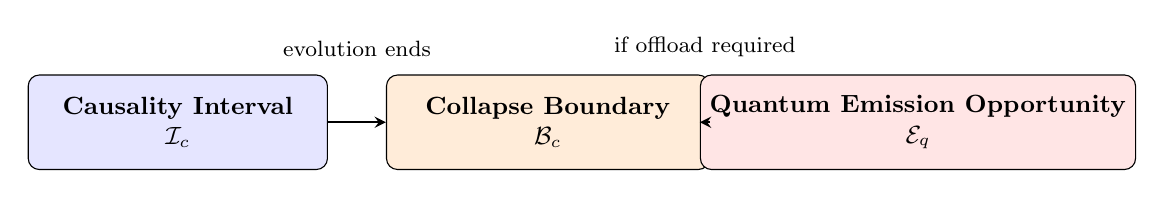
\begin{tikzpicture}[>=stealth, node distance=4.7cm, every node/.style={font=\small}, align=center]

% Nodes
\node (ci) [draw, rounded corners, minimum width=3.8cm, minimum height=1.2cm, fill=blue!10] {\textbf{Causality Interval} \\ \( \mathcal{I}_c \)};
\node (cb) [right of=ci, draw, rounded corners, minimum width=4.1cm, minimum height=1.2cm, fill=orange!15] {\textbf{Collapse Boundary} \\ \( \mathcal{B}_c \)};
\node (qeo) [right of=cb, draw, rounded corners, minimum width=4.3cm, minimum height=1.2cm, fill=red!10] {\textbf{Quantum Emission Opportunity} \\ \( \mathcal{E}_q \)};

% Arrows
\draw[->, thick] (ci) -- (cb) node[midway, above, yshift=2.0em] {\footnotesize evolution ends};
\draw[->, thick] (cb) -- (qeo) node[midway, above, yshift=2.0em] {\footnotesize if offload required};

% Labels under nodes
%\node at ($(ci.south) + (0,-0.3)$) {\footnotesize quantum evolution (unitary)};
%\node at ($(cb.south) + (0,-0.3)$) {\footnotesize structure re-locks};
%\node at ($(qeo.south) + (0,-0.3)$) {\footnotesize serialized emission};

\end{tikzpicture}
\caption{CI–CB–QEO sequence within a coherence frame. Quantum behavior occurs within the Causality Interval \( \mathcal{I}_c \), terminates at the Collapse Boundary \( \mathcal{B}_c \), and may emit a signal at the Quantum Emission Opportunity \( \mathcal{E}_q \).}
\label{fig:cicbqeo}
\end{figure}



We conclude by identifying testable observational signatures—such as nucleation thresholds, CPA drag, and shell-band spectra—and propose that mass is not a parameter but a structural outcome: the causal residue of what the substrate allows to persist.
\footnote{For detailed experimental predictions and observables, see Appendix~\ref{app:experimental}.}
%%%%%%%%%%%%%%%%%%%%%%%%%%%%%%%%%%%%%%%%%%

%%%%%%%%%%%%%%%%%%%%%%%%%%%%%%%%%%%%%%%%%%
\section{Materials and Methods}
%%%%%%%%%%%%%%%%%%%%%%%%%%%%%%%%%%%%%%%%%%
\qsdmethodstatement
\\
In support of the editorial process, generative AI tools—specifically OpenAI's ChatGPT (version 5, 2025)—were used to assist in:
\begin{itemize}
    \item Generating initial illustrative figures based on the author’s conceptual framework
    \item Refining the typesetting, language, grammar and spelling.
\end{itemize}

No original theoretical contributions were generated by the AI system; all scientific claims, hypotheses, derivations, and interpretations were authored and reviewed by the human researcher. The use of AI is disclosed in alignment with journal policy for transparency in the writing process.

%%%%%%%%%%%%%%%%%%%%%%%%%%%%%%%%%%%%%%%%%%
%\section{Results}

%%%%%%%%%%%%%%%%%%%%%%%%%%%%%%%%%%%%%%%%%%
\section{Discussion}
%%%%%%%%%%%%%%%%%%%%%%%%%%%%%%%%%%%%%%%%%
\subsection{Substrate Law and the Collapse Boundary (CB)}

In Quantum Substrate Dynamics (QSD), the evolution of matter and fields is not governed by external geometry or imposed force, but by the internal limits of a conserved Lorentz-invariant substrate. This substrate advances in discrete \emph{Causality Intervals} (CI), each terminating at a \emph{Collapse Boundary} (CB). The CB is the structural checkpoint where unresolved energy or deformation must be reconciled to preserve coherence. It is not an optional event; it is the deterministic enforcement of the substrate’s finite capacity.

\subsubsection*{Deterministic Enforcement of Coherence}

The CB embodies what we term the \emph{substrate law}: coherence must be restored before the next interval begins. The requirement is structural, not probabilistic. By the end of each CI, the local region must resolve into one of the permitted states. If alignment cannot be recovered, the system defaults to one of four causal pathways: (i) radiative emission, (ii) geometric reconfiguration (momentum transfer), (iii) rupture, or (iv) phase capture into a persistent mass nucleus.

\subsubsection*{Unified Resolution Bounds}

All four pathways are governed by the same feasibility conditions:
\begin{equation}
\frac{\Delta E}{\tau} \leq \min\{c^5,\,P_{\text{avail}}\}, \qquad
\Delta E < E_{\mathrm{P}}(L) = \frac{c_t^4}{G}L, \qquad
A_\kappa(L) \leq \eta A_{\max}, \qquad
\Gamma \in [0,1],
\end{equation}
where:
\begin{itemize}
    \item \( \Delta E \): unresolved energy awaiting dissipation or capture,
    \item \( \tau = L_{\mathrm{coh}} / c_s \): scalar pacing interval for the CI,
    \item \( c_t, c_s \): transverse and scalar propagation rates,
    \item \( G \): substrate curvature compliance,
    \item \( E_{\mathrm{P}}(L) \): maximum yield energy for scale \( L \),
    \item \( A_\kappa(L) \): action required to sustain a structure of complexity \( \kappa \),
    \item \( A_{\max} = E_{\mathrm{P}}\tau \equiv h \): coherence–information capacity (CIC),
    \item \( \eta \in (0,1] \): structural efficiency,
    \item \( \Gamma \): overlap fraction of coherence modes.
\end{itemize}

The dominant constraint dictates the outcome: failed overlap produces emission, excess energy density forces rupture, complexity exceeding CIC dissolves, and compliance within all bounds allows nucleation.

\subsubsection*{Causal Centrality of the CB}

Each CB enforces this substrate law universally—there are no exceptions for particle type, interaction channel, or observer context. Photons, momentum exchange, rupture events, and mass genesis all resolve through the same finite-capacity criteria. The CB is thus the causal fulcrum of physical law, the point where coherence either resets, redistributes, or persists.

\subsubsection*{Reframing Quantum Evolution}

In this view, quantum collapse is not a probabilistic jump or observer-induced reduction, but a deterministic reconfiguration governed by finite coherence capacity. The substrate law replaces indeterminacy with structural necessity: radiation, motion, and mass all arise as direct outcomes of the same bounded feasibility conditions. This unifies emission, inertia, and nucleation under a single physical principle of coherence conservation.


%%%%%%%%%%%%%%%%%%%%%%%%%%%%%%%%%%%%%%%%%%
\subsection{Collapse Resolution and the Origin of Mass}

In QSD, mass is not a primitive entity but the most durable resolution of coherence under collapse pressure. At the end of every \emph{Causality Interval} (CI), a region of the substrate must resolve its structural state at a \emph{Collapse Boundary} (CB). This resolution event—termed a \emph{Quantum Emission Opportunity} (QEO)—is compulsory, enforced by the finite coherence support of the substrate. All observable outcomes at this point—radiation, momentum transfer, rupture, or mass-phase capture—emerge from a single feasibility condition.

\subsubsection*{Unified Collapse Constraint}

At the CB, the system evaluates whether the configuration can be recovered within the allowable coherence window. This is formalized as a feasibility set:
\begin{equation}
\frac{\Delta E}{\tau} \leq \min\{c^5,\,P_{\mathrm{avail}}\}, \quad
\Delta E < E_{\mathrm{P}}(L) = \frac{c_t^4}{G}L, \quad
A_\kappa(L) \leq \eta A_{\max}(L), \quad
\Gamma \in [0,1],
\label{eq:collapse_constraints}
\end{equation}
where:
\begin{itemize}
\item \( \Delta E \) is the unresolved residual energy,
\item \( \tau = \frac{L_{\mathrm{coh}}}{c_s} \) is the scalar pacing interval,
\item \( c_t \) and \( c_s \) are the transverse and scalar coherence propagation rates,
\item \( G \) is the substrate curvature compliance constant,
\item \( A_\kappa(L) \) is the per-tick structural action for a configuration of complexity \( \kappa \),
\item \( \eta \in (0,1] \) is the coherence retention efficiency,
\item \( \Gamma \) is the phase-overlap fraction,
\item \( A_{\max}(L) = E_{\mathrm{P}}(L)\cdot\tau \equiv h \) is the coherence–information capacity (CIC).
\end{itemize}

Each outcome follows from the dominant constraint. Failed overlap yields radiation, excess energy density produces rupture, and successful retention within the CIC permits persistence.

\subsubsection*{Mass as Persistent Collapse Lock}

When the substrate resolves a CB by forming a structure that survives across multiple intervals without exceeding yield or complexity thresholds, a \emph{mass-phase nucleus} is established. This marks the transition from transient coherence to persistent inertia. Such a nucleus is not “stored mass” in the classical sense but a locked phase configuration resistant to dissolution by virtue of compatibility with the coherence envelope. Mass is, in this framework, \emph{the structure coherence locks into when no escape path is feasible}.

\subsubsection*{Planck Threshold as Nucleation Gate}

The storage ceiling is set by the yield constraint,
\[
E_{\mathrm{P}}(L) = \frac{c_t^4}{G}L.
\]
This specifies the maximum energy a coherence envelope of scale \( L \) can support without rupture. Combined with the scalar pacing interval, the maximum recoverable action is
\[
A_{\max}(L) = E_{\mathrm{P}}(L)\cdot\tau = \frac{c_t^4}{c_s}\cdot\frac{L^2}{G}.
\]
This represents the geometric and dynamical origin of Planck’s constant in QSD: the action budget per causal interval.

The critical transition to mass-phase occurs when the coherence packet:
\begin{enumerate}
\item cannot emit fast enough (\( \Delta E/\tau > P_{\mathrm{avail}} \)),
\item cannot geometrically reorganize,
\item remains below the rupture threshold,
\item lies within the CIC “Goldilocks window” permitting structural re-lock.
\end{enumerate}

At this point, the collapse boundary locks into a configuration that persists across intervals. Mass thus appears as the durable residue of coherence that cannot be undone.\footnote{For an analytical illustration of how these constraints define a critical feasibility wedge, see Appendix~\ref{app:toy}.}

\subsubsection*{Mass as Dimensional Anchor}

A mass-phase nucleus anchors its region of space to a defined coherence state. Dissolution requires external input exceeding both yield and pacing bounds. Mass therefore functions as a dimensional knot in the substrate field—a durable avoidance of rupture.

\subsubsection*{Implications for Mass Genesis}

Mass genesis is emergent, not additive. The substrate cannot accumulate mass arbitrarily but only under specific yield, pacing, and complexity bounds. This explains the discreteness of matter, the stability of nuclei, and the termination of fusion beyond iron-group elements. Once a configuration saturates its Planck envelope, the system either emits, ruptures, or locks. See Figure \ref{fig:collapse_flowchart}.

Accordingly, the origin of mass is not attributed to virtual couplings (e.g., Higgs) but to the physical refusal of coherence to yield, stabilized by geometry and pacing constraints. Each atom is a stable collapse solution.



\tikzstyle{startstop} = [rectangle, draw=black, fill=gray!10, minimum width=5cm, minimum height=1cm, text centered]
%\tikzstyle{decision} = [diamond, draw=black, fill=blue!10, minimum width=4.5cm, minimum height=2.5cm, text centered, aspect=2]
\tikzstyle{decision} = [rectangle, draw=black, fill=blue!10, minimum width=6.5cm, minimum height=1cm, text centered]

\tikzstyle{outcome} = [rectangle, draw=black, fill=green!10, minimum width=3.5cm, minimum height=1cm, text centered]
\tikzstyle{arrow} = [thick, ->, >=Stealth]

\begin{figure}[h!]
\centering
\begin{tikzpicture}[node distance=2cm]

% Nodes
\node (start) [startstop] {Collapse Boundary Reached};

\node (yield) [decision, below of=start, align=center] 
  {Yield Constraint $\Delta E < E_{\mathrm{P}}(L)$?};
\node (action) [decision, below of=yield, align=center] {Maintenance Constraint
$A_\kappa \leq \eta A_{\max}$?};
\node (geometry) [decision, below of=action, align=center] {Geometric Overlap 
$\Gamma \sim 1$?};

\node (rupture) [outcome, right=4.5cm of yield] {Rupture};
\node (bleed) [outcome, right=4.5cm of action] {Coherence Bleed};
\node (emit) [outcome, right=4.5cm of geometry] {Radiative Emission};
\node (mass) [outcome, below=2cm of geometry] {Mass-Phase Capture};

% Arrows (yes paths)
\draw [arrow] (start) -- (yield);
\draw [arrow] (yield) -- node[left] {Yes} (action);
\draw [arrow] (action) -- node[left] {Yes} (geometry);
\draw [arrow] (geometry) -- node[left] {Yes} (mass);

% Arrows (no paths to outcomes)
\draw [arrow] (yield.east) -- ++(1,0) -- (rupture.west) node[midway, above] {No};
\draw [arrow] (action.east) -- ++(1,0) -- (bleed.west) node[midway, above] {No};
\draw [arrow] (geometry.east) -- ++(1,0) -- (emit.west) node[midway, above] {No};

\end{tikzpicture}
\caption{Collapse Outcome Flowchart. At each Collapse Boundary, the substrate evaluates yield, action, and geometric constraints to determine whether the structure ruptures, bleeds, emits, or becomes a stable mass-phase nucleus.}
\label{fig:collapse_flowchart}
\end{figure}


%%%%%%%%%%%%%%%%%%%%%%%%%%%%%%%%%%%%%%%%%%
\subsection{Collapse-Resolved Mass Structures}

The Quantum Substrate Dynamics (QSD) framework derives mass-phase structures not from particle postulates or symmetry breaking, but from structural survival under collapse constraints. To formalize this, we construct an action-based model that embeds the feasibility bounds of collapse resolution into a variational substrate law.

This section refines the substrate action principle specifically to frame mass persistence as a stable solution to causal pacing, structural yield, and coherence capacity constraints. The action is not abstract—it is the governing currency that determines which coherence structures survive and which collapse.

\subsubsection*{Interval-Defined Action Domain}

Each region of the substrate evolves within discrete \emph{Causality Intervals} (CI) of duration 
\[
\tau = \frac{L_{\mathrm{coh}}}{c_s}.
\]
The action accrued during one interval is given by:
\begin{equation}
\mathcal{S} = \int_{t}^{t+\tau} \mathcal{L}(\psi, \partial_t \psi, \nabla \psi; L_{\mathrm{coh}})\, dt,
\end{equation}
where \( \psi \) is the local coherence field over the region defined by \( L_{\mathrm{coh}} \), and \( \mathcal{L} \) is the Lagrangian density capturing coherence dynamics.

\subsubsection*{Mass-Relevant Lagrangian Structure}

The Lagrangian is structured to reflect the substrate’s physical limits:
\begin{equation}
\mathcal{L} = \frac{1}{2}\left(\frac{\partial_t \psi}{c_s}\right)^2 
- \frac{1}{2}\left(\frac{\nabla \psi}{c_t}\right)^2 
- V(\psi, \nabla \psi; L_{\mathrm{coh}}),
\end{equation}
with:
\begin{itemize}
  \item \( c_s \): scalar recovery speed setting tick duration,
  \item \( c_t \): transverse coherence propagation rate,
  \item \( V \): effective potential encoding rupture thresholds, complexity saturation, and CPA distortions.
\end{itemize}

This structure reflects local phase inertia, coherence drag, and constraint-induced geometric suppression—all of which affect whether a configuration survives collapse.

\subsubsection*{Variational Collapse Filter}

Applying the principle of stationary action over each CI yields:
\begin{equation}
\frac{\partial^2 \psi}{\partial t^2} 
- \left(\frac{c_s}{c_t}\right)^2 \nabla^2 \psi 
+ c_s^2 \frac{\partial V}{\partial \psi} = 0.
\end{equation}
This field equation governs collapse evolution. When paired with the Planck action bound:
\begin{equation}
\int_{t}^{t+\tau} \mathcal{L}\, dt \;\leq\; h,
\end{equation}
it creates a **causal sieve**—only those configurations whose structural complexity, coherence drag, and curvature energy remain within the substrate’s pacing budget can survive.

\subsubsection*{Action as a Mass Selection Operator}

This formalism links directly to the feasibility inequalities used in the prior section. The complexity-weighted action \( A_\kappa \), the yield threshold \( E_{\mathrm{P}}(L) \), and the coherence–information capacity \( A_{\max} \) all emerge as **evaluated integrals of this Lagrangian form** over the coherence domain.

A configuration that:
\[
\text{minimizes } \mathcal{S} \quad \text{and} \quad \mathcal{S} \leq h
\]
persists as a mass-phase nucleus. All others—those requiring excessive internal action or exceeding yield—must rupture or dissipate.

\subsubsection*{From Structure to Quantization}

Quantized mass spectra emerge because only a **finite set of internal waveform geometries** satisfy the stationarity condition under bounded \( \mathcal{S} \). The discreteness of matter is not postulated—it is selected by the substrate’s collapse gate, governed by this action integral.

Thus, the action principle is not an external mathematical overlay but the **intrinsic enforcement rule of the substrate**. Mass survives because it fits within the allowable structural evolution budget of each tick. This frames mass as a viable coherence path through collapse—not a primitive input, but the filtered output of constrained causal geometry.

%%%%%%%%%%%%%%%%%%%%%%%%%%%%%%%%%%%%%%%%%%
\subsection{Collapse Constraints and the Feasibility Window for Mass Persistence}

In Quantum Substrate Dynamics (QSD), mass is not a fundamental input, but an outcome of coherence survival under collapse constraints. Each region of the substrate evolves in discrete \emph{Causality Intervals} (CI), terminating at a \emph{Collapse Boundary} (CB). At this CB, the system must resolve its coherence structure. Permitted outcomes include emission (offload), rupture, geometric momentum transfer, or persistent re-locking. Mass-phase nucleation corresponds to this final case: a configuration that successfully locks into the substrate and persists across intervals.

\subsubsection*{Feasibility Inequalities: Collapse Constraint Window}

Persistence is permitted only when two substrate constraints are simultaneously satisfied:

\begin{equation}
A_\kappa(L) \leq \eta\,A_{\max}(L), 
\qquad 
\Delta E < E_{\mathrm{P}}(L) = \frac{c_t^4}{G}\,L.
\end{equation}

\begin{itemize}
    \item The \textbf{maintenance constraint} requires that the per-tick action to preserve a structure of complexity \( \kappa \) remain below the coherence–information capacity (CIC), \( A_{\max}(L) \).
    \item The \textbf{yield constraint} enforces that unresolved energy at collapse stays below the rupture threshold \( E_{\mathrm{P}}(L) \).
\end{itemize}

Structures outside this bounded wedge either emit, rupture, or dissipate. Only those within the window can persist through repeated CI--CB cycles.

\subsubsection*{Mass as Coherence-Locked Resolution}

Mass, in this framework, is not “stored energy” or the result of external interaction fields. It is a stable, causally permitted configuration that survives the CB re-locking process. This structural survival requires internal symmetry, reduced action burden, and compatibility with the local substrate’s pacing and compliance.

The apparent permanence of mass arises not from intrinsic properties, but from sustained feasibility under the substrate's resolution law. Mass is thus defined as the most durable offload structure the substrate can support, not as a fixed ontological category.

\subsubsection*{Scale Dependence, Discreteness, and the Nucleation Threshold}

The feasibility window is not scale-invariant. Because the CIC and yield bounds scale as:
\[
A_{\max} \propto L^2, \quad E_P \propto L,
\]
only structures above a critical size \( L_n \) can survive. Below this threshold, coherence cannot be retained—the action is too high or the yield too low. This creates a \textbf{natural discreteness} in allowed mass configurations. The substrate itself selects which structures persist.

\subsubsection*{Local Saturation and Collapse Suppression}

Substrate capacity is locally variable. Regions saturated with locked coherence or unrecovered scalar memory resist new locking. This is modeled by promoting curvature compliance \( G \) and other parameters to effective, position-dependent fields:

\[
G \rightarrow G_{\mathrm{eff}}(\mathbf{x},t) = G_0\,\mathcal{G}(\rho_M, R, \nabla\theta),
\]

where:
\begin{itemize}
    \item \( \rho_M \): local mass-phase density,
    \item \( R \): scalar recovery field,
    \item \( \nabla\theta \): phase curvature or memory drag.
\end{itemize}

Other CI-coupled parameters follow:
\[
c_s \rightarrow c_{s,\mathrm{eff}}, \quad 
\eta \rightarrow \eta_{\mathrm{eff}}, \quad 
\Gamma \rightarrow \Gamma_{\mathrm{eff}}.
\]

These modify the collapse inequalities accordingly:

\begin{align}
\frac{\Delta E}{\tau_{\mathrm{eff}}} &\le \min\{c^5, P_{\mathrm{avail}}\}, \qquad 
\tau_{\mathrm{eff}} = \frac{L}{c_{s,\mathrm{eff}}}, \\[4pt]
\Delta E &< \frac{c_t^4}{G_{\mathrm{eff}}}\,L, \\[4pt]
A_\kappa &\le \eta_{\mathrm{eff}}\,\frac{c_t^4}{c_{s,\mathrm{eff}}\,G_{\mathrm{eff}}}\,L^2.
\end{align}

\paragraph{Exclusion Corollary (Conservation-Based Suppression).}

When coherence is already locked or unrecovered, nucleation is structurally excluded. This is not an imposed rule, but a natural outcome of conservation:

\[
G_{\mathrm{eff}} \downarrow, \quad c_{s,\mathrm{eff}} \downarrow, \quad \eta_{\mathrm{eff}} \downarrow 
\;\Rightarrow\; A_\kappa > \eta_{\mathrm{eff}}\,A_{\max}^{\mathrm{loc}} \;\Rightarrow\; \text{no locking}.
\]

This directly explains why no new mass forms in dense solids or coherence-saturated regions.

\subsubsection*{Inertial Implications and Structural Memory}

A mass-phase structure retains its configuration across intervals without external stabilization. Inertia in QSD arises from this locked structural persistence---dragged forward only by coherence re-locking in the same configuration. Local gradients or CPA memory fields affect feasibility, creating resistance to acceleration or redirection.

\subsubsection*{Unified View: Collapse Constraints Define Mass}

This framework provides a unified causal account for:
\begin{itemize}
    \item why mass appears,
    \item where it cannot appear,
    \item why it is discrete,
    \item and why it persists.
\end{itemize}

Mass is what remains when all other collapse paths are unavailable, and structure can re-lock under bounded action and yield. It is the residue of structural success, not a primitive variable.

\subsubsection{Empirical Boundary}
\paragraph{Iron-Group Nucleation Cutoff}

The derived collapse constraints in QSD imply a natural ceiling on mass-phase nucleation, enforced by the Planck action limit and structural feasibility bounds. Remarkably, this limit corresponds precisely with a well-known empirical cutoff in stellar fusion: the iron group.

In stellar interiors, fusion reactions release energy only up to the formation of iron-56. Beyond this, fusion becomes endothermic—requiring more energy input than it provides in binding energy. Within the QSD framework, this transition marks the point where nucleated coherence structures exceed the substrate’s causal action budget per tick. The structural action \( A_\kappa \) required to stabilize heavier nuclei breaches the feasibility window defined by:
\[
A_\kappa(L) \leq \eta\,A_{\max}(L), \quad \Delta E < \frac{c_t^4}{G}\,L.
\]

As nucleon complexity and internal waveform curvature increase beyond iron, so too does the required action. Eventually, the system reaches a point where it must rupture or emit—new locking is no longer structurally viable under the collapse constraints.

This explains why fusion halts at iron under normal conditions. Heavier elements are observed, but only as products of supernovae or neutron-star collisions—high-energy collapse events that temporarily bypass the standard pacing and yield gates. These events momentarily unlock new portions of the feasibility landscape by increasing available energy and reducing local compliance thresholds.

QSD therefore grounds the iron fusion ceiling as a direct consequence of collapse-bound structural physics. This observation does not merely coincide with the theory—it validates its quantitative collapse gating as physically realized in stellar evolution.

\paragraph{Supernova Collapse and Structural Access to Heavy Element Locking}

While standard stellar fusion terminates at the iron group due to insufficient feasibility headroom in the substrate, quantum substrate dynamics (QSD) predicts that higher mass-phase locking becomes viable in collapse environments where local parameters transiently expand the collapse constraint window.

During core-collapse supernovae, extreme compression followed by violent re-expansion drives coherent shock fronts through the substrate. This temporarily alters the local coherence environment in two principal ways:
\begin{enumerate}
    \item The effective coherence length \( L_{\mathrm{coh}} \) increases dramatically due to macroscopic field compression and energy concentration.
    \item The scalar recovery rate \( c_s \) drops momentarily behind the shock interface, delaying re-lock and extending the causal interval \( \tau = L_{\mathrm{coh}} / c_s \).
\end{enumerate}

Together, these effects dynamically increase the available action and yield budgets:
\begin{align}
A_{\max}^{\mathrm{loc}} &= \frac{c_t^4}{G_{\mathrm{eff}}\,c_{s,\mathrm{eff}}}\,L_{\mathrm{coh}}^2, \\[6pt]
E_P^{\mathrm{loc}} &= \frac{c_t^4}{G_{\mathrm{eff}}}\,L_{\mathrm{coh}}.
\end{align}

This creates a brief window in which:
\begin{itemize}
    \item Structures with higher internal complexity \( \kappa \),
    \item and larger residual energy \( \Delta E \)
\end{itemize}
can be resolved as mass-phase nuclei without exceeding the feasibility limits. In essence, the substrate “stretches” its nucleation capacity during this dynamic rupture–recovery process.

Such a mechanism naturally explains the formation of post-iron elements during supernovae—an observational fact long recognized in astrophysics. Under QSD, these elements are not produced by brute-force accumulation, but by temporarily satisfying the same collapse conditions as lighter mass structures—using a locally elevated feasibility envelope.

This offers a concrete grounding of the QSD framework in empirical nucleosynthetic behavior, without violating the conserved substrate principles or requiring new rules.


%%%%%%%%%%%%%%%%%%%%%%%%%%%%%%%%%%%%%%%%%%
\begin{tcolorbox}[colback=gray!5!white, colframe=black!50!black, title={Empirical Anchors for Collapse-Driven Mass Nucleation}]
Quantum Substrate Dynamics (QSD) does not modify known observational outcomes—it structurally explains them. The collapse-resolution model for mass persistence aligns naturally with key empirical features of matter genesis:

\begin{itemize}
    \item \textbf{Iron Fusion Ceiling:} Fusion halts at iron-group elements because structural retention constraints (yield + action) become saturated beyond this point. QSD derives this limit from the Planck-bound collapse feasibility window.
    
    \item \textbf{Supernova Nucleosynthesis:} Heavier-than-iron nuclei form only when a supernova injects sufficient coherence action and compression (\( \Delta E \uparrow \), \( L_{\mathrm{coh}} \uparrow \)) into a rapidly recovering substrate. QSD models this as collapse boundary locking under shock-inflated feasibility windows.

    \item \textbf{Isotopic Abundance Patterns:} The nonuniform distribution of stable isotopes across mass number reflects the discrete action-valid configurations permitted by collapse geometry. QSD accounts for this as a structural selection filter under bounded action.

    \item \textbf{Neutron Star Matter and CI-Saturation:} Inertial drag, collapse density, and CPA saturation are consistent with the suppression of new locking in highly compact environments. QSD frames this suppression as conservation-driven exclusion from already committed coherence.

\end{itemize}

\vspace{4pt}
These alignments are not retrofits—they follow necessarily from the collapse constraints embedded in QSD. No parameter tuning or external assumptions are required.
\end{tcolorbox}

%%%%%%%%%%%%%%%%%%%%%%%%%%%%%%%%%%%%%%%%%%
\subsection{Minimal Mass-Phase Locks and the Origin of Elemental Abundances}

The collapse constraints discussed above not only define the general feasibility of mass-phase persistence, but also explain why certain mass configurations—such as protons and electrons—dominate the observed universe. These structures represent the ground state of substrate-locking: the simplest, most stable solutions that satisfy all feasibility conditions under collapse pressure.

Within Quantum Substrate Dynamics (QSD), mass-phase nucleation occurs when a coherence structure satisfies the full set of substrate constraints—action, yield, pacing, and geometric overlap—within a single Causality Interval (CI). The lowest-energy configurations capable of surviving a Collapse Boundary (CB) define the lower edge of the \emph{Goldilocks window} for persistence. These are the \emph{minimum-lockable mass structures}. See Figure \ref{fig:feasibility_wedge}.

Hydrogen nuclei and free electrons appear to occupy this minimal stability zone. Their ubiquity is not merely a consequence of thermal processes or Big Bang nucleosynthesis, but—within the QSD framework—a reflection of structural compatibility. These configurations require the least internal action to maintain, remain well below rupture thresholds, and exhibit sufficient spatial symmetry to support high overlap probability (\( \Gamma \sim 1 \)). In this view, they are not just relics of early cosmology but dynamically preferred solutions selected by the substrate’s collapse law.

\begin{figure}[h!]
\centering
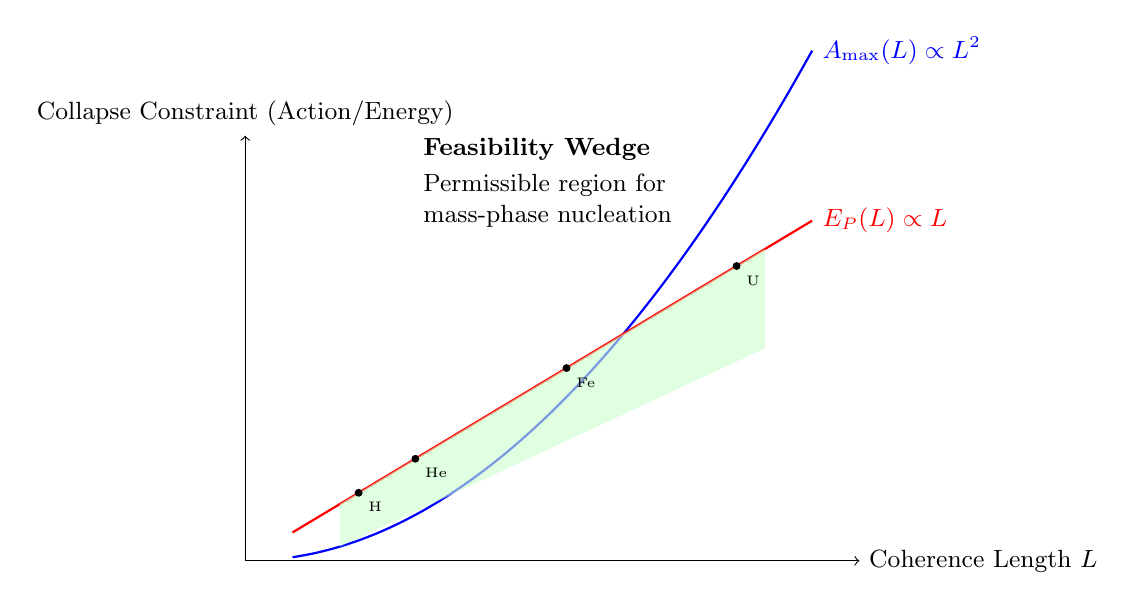
\begin{tikzpicture}[scale=1.2]

% Axes
\draw[->] (0,0) -- (6.5,0) node[right] {\small Coherence Length $L$};
\draw[->] (0,0) -- (0,4.5) node[above] {\small Collapse Constraint (Action/Energy)};

% Constraint curves
\draw[thick,blue,domain=0.5:6,smooth,variable=\x] plot ({\x},{0.15*\x*\x}) node[right,blue] {\small $A_{\max}(L) \propto L^2$};
\draw[thick,red,domain=0.5:6,smooth,variable=\x] plot ({\x},{0.6*\x}) node[right,red] {\small $E_P(L) \propto L$};

% Fill feasibility wedge (approximate polygon)
\fill[green!20,opacity=0.6]
  (1,0.6) --
  (5.5,3.3) --
  (5.5,2.25) --
  (1,0.15*1*1) -- cycle;

% Example element points
\draw[fill=black] (1.2,0.72) circle (1pt) node[below right] {\tiny H};
\draw[fill=black] (1.8,1.08) circle (1pt) node[below right] {\tiny He};
\draw[fill=black] (3.4,2.04) circle (1pt) node[below right] {\tiny Fe};
\draw[fill=black] (5.2,3.12) circle (1pt) node[below right] {\tiny U};

% Annotation
\node[align=left, font=\small] at (3.2,4) {\textbf{Feasibility Wedge}\\[2pt]
Permissible region for\\
mass-phase nucleation};

\end{tikzpicture}
\caption{Collapse feasibility wedge bounded by the maintenance constraint ($A_{\max}(L)$) and yield constraint ($E_P(L)$). Element labels indicate relative positions of stable structures that satisfy QSD nucleation criteria.}
\label{fig:feasibility_wedge}
\end{figure}


This provides a causal reinterpretation of elemental abundance distributions. Rather than being solely governed by nuclear or chemical pathways, the persistence of different elements follows from their ability to satisfy collapse constraints under local substrate conditions. Higher-mass nuclei demand greater precision in action balance and are less likely to persist unless supported by favorable compression, phase wake, or CPA memory structures. In contrast, hydrogen and electrons dominate in low-curvature regions where only minimal locking is viable.

The prevalence of these simple structures—especially in interstellar and intergalactic media—offers a structural insight: the universe remains filled with the most coherence-compatible mass locks. They form a stable background lattice from which more complex nuclei emerge only when local substrate gradients permit. In this framing, abundance becomes a probabilistic occupancy of feasible collapse solutions—not an outcome of equilibrium chemistry, but a reflection of collapse dynamics under constraint.

\begin{tcolorbox}[colback=black!4, colframe=black!30!black, title=Structural Basis for Elemental Abundance]
Hydrogen nuclei and free electrons persist because they lie within the minimal feasible region of the collapse constraint wedge. Their coherence demands are low, symmetry is high, and re-locking probability approaches unity. Their cosmic abundance reflects structural compatibility, not just thermodynamic origin.
\end{tcolorbox}


%%%%%%%%%%%%%%%%%%%%%%%%%%%%%%%%%%%%%%%%%%
\subsection{Collapse-Emergent Gravity: Compliance Gradients as Effective Geometry}

Gravitational behavior in Quantum Substrate Dynamics (QSD) emerges not from spacetime curvature, but from structural gradients in substrate compliance. As collapse-locked mass-phase nuclei form, they consume local coherence capacity—modulating the substrate’s ability to support transverse reconfiguration. This modulation creates spatial differentials in recovery pacing and offload feasibility, biasing surrounding coherence flows toward the mass center.

In this framework, the gravitational constant \( G \) is recast as a substrate yield coefficient—a measure of how much transverse phase deformation the substrate can support before rupture or phase-locking occurs. This yield is not uniform: local saturation, scalar recovery lag, and residual memory gradients all alter the effective compliance, creating a causal geometry from structural limits.

We formalize this with the compliance field:
\[
\mathcal{C}(\mathbf{x},t) = \frac{1}{G_{\mathrm{eff}}(\mathbf{x},t)},
\]
where \( G_{\mathrm{eff}} \) reflects position-dependent substrate properties:
\begin{itemize}
    \item \( \rho_M \): coherence saturation from local mass-phase density,
    \item \( R \): scalar recovery capacity, and
    \item \( \nabla \theta \): phase curvature and CPA-induced drag.
\end{itemize}

Gradients in \( \mathcal{C} \) define preferred directions of phase propagation—replacing the geodesic paths of general relativity with steepest-descent coherence trajectories. Motion occurs not because of force, but because substrate stability is biased toward regions of greater re-lock feasibility.

This structural reinterpretation naturally reproduces gravitational redshift, time dilation, and lensing as outcomes of coherence timing and compliance saturation—not as warps in spacetime. An effective metric emerges from substrate deformation:
\[
g_{\mu\nu}^{\mathrm{eff}} = \eta_{\mu\nu} + \delta_{\mu\nu}(\nabla \mathcal{C}),
\]
mirroring general relativity's geometry while exposing a causal substrate origin. In high-curvature regimes or coherence-dense environments, this substrate-driven model predicts measurable departures from GR, grounded in action conservation and recovery pacing.

In total, collapse-emergent gravity arises from the same substrate dynamics that define mass persistence. Gravity is not added to QSD—it is a consequence of structural bias left in the substrate after re-locking.

%%%%%%%%%%%%%%%%%%%%%%%%%%%%%%%%%%%%%%%%%%
\subsection{Collapse-Driven Thermodynamics: Entropy Flow in a Coherence-Limited Medium}

Just as structural saturation drives gravity, it also defines the thermodynamic flow of entropy in Quantum Substrate Dynamics. Each \emph{Collapse Boundary} (CB) represents an irreversible event—a point at which unresolved energy and phase structure must be reconciled within a finite coherence budget. These reconciliations are not merely energetic; they are structural transitions with measurable entropic consequences.

Substrate entropy in QSD is a function of coherence mode overlap:
\begin{equation}
S_{\mathrm{QSD}} \propto - \int \Gamma(x,t)\, \log \Gamma(x,t) \;\mathrm{d}x,
\end{equation}
where \( \Gamma \in [0,1] \) is the local phase-overlap field. When coherence dissolves, entropy increases; when structure persists or re-locks, entropy decreases. This reframes entropy not as disorder, but as a measure of uncommitted phase potential.

Collapse outcomes yield distinct entropic signatures:
\begin{itemize}
    \item \textbf{Emission}: increases entropy by shedding unresolvable phase via radiation.
    \item \textbf{Rupture}: maximizes entropy through loss of coherence support.
    \item \textbf{Bleed}: slowly raises entropy via coherence dissipation.
    \item \textbf{Nucleation}: reduces entropy by locking structure and restoring overlap.
\end{itemize}

These outcomes are determined by the same feasibility bounds that govern mass and gravity—there is no separate thermodynamic layer. Entropy flow is the cumulative record of structural resolution under finite action constraints.

Collapse dynamics are inherently time-asymmetric. The evolution within a CI proceeds forward, but the resolution at the CB defines an irreversible projection. CPA (Causal Phase Aftereffect) fields store memory of past collapse geometry, biasing future locking and offload. This causes directional asymmetries in entropy flow, including:
\begin{itemize}
    \item emission rings and echo shells,
    \item coherence drag shadows,
    \item entropy accumulation in CPA-saturated zones.
\end{itemize}

Each CB enforces a local action bound:
\[
\int_{t}^{t+\tau} \mathcal{L} \, dt \le h,
\]
limiting entropy production per interval. This substrate constraint throttles thermal flow—entropy cannot grow faster than the coherence budget allows. In high-density regions, this bottleneck explains delayed phase transitions or rupture events. In low-density zones, it explains entropy cycling and structure retention.

Under QSD, entropy is not a statistical artifact but a structural currency—expended or conserved through collapse resolution. The thermodynamic arrow of time emerges not from probabilistic tendencies, but from irreversible coherence decisions enforced by collapse topology.




%%%%%%%%%%%%%%%%%%%%%%%%%%%%%%%%%%%%%%%%%%
\subsection{Substrate Yield as Structural Collapse Threshold}

Mass-phase persistence in QSD is bounded not by external forces or particle potentials, but by the internal structural capacity of the substrate to retain coherence under finite curvature tension. This limit is expressed through the concept of \textit{substrate yield}—a scale-dependent upper bound on the unresolved energy that can remain stored within a coherence envelope without inducing rupture.

\subsubsection*{Planck Yield Bound}

The substrate yield threshold is defined by a generalized Planck-like expression:
\begin{equation}
E_{\mathrm{P}}(L) = \frac{c_t^4}{G}\,L,
\label{eq:substrate-yield}
\end{equation}
where:
\begin{itemize}
    \item \( c_t \) is the transverse coherence propagation speed (controlling phase spread),
    \item \( G \) is the substrate curvature compliance constant (governing structural resistance),
    \item \( L \) is the spatial scale of the coherence packet.
\end{itemize}

This bound represents the maximum energy that a coherence structure of size \( L \) can sustain without exceeding the substrate’s local support capacity. It defines a rupture horizon: if the unresolved energy \( \Delta E \) at a \emph{Collapse Boundary} (CB) exceeds \( E_{\mathrm{P}}(L) \), structural compatibility fails and rupture must occur. No stabilization or emission pathway remains feasible.

\subsubsection*{Action Limit and Coherence–Information Capacity}

The yield constraint directly governs the allowable action per \emph{Causality Interval} (CI). The maximum structural action is:
\begin{equation}
A_{\max}(L) = E_{\mathrm{P}}(L)\,\tau = \frac{c_t^4}{c_s} \cdot \frac{L^2}{G},
\end{equation}
where \( \tau = L/c_s \) is the scalar recovery interval. This defines the \emph{coherence–information capacity} (CIC): the total re-lockable structural budget of a coherence region per causal cycle.

This action bound is not an external constraint—it arises from substrate conservation. Each region can only process a finite amount of internal structural evolution per interval, regardless of excitation history. The Planck constant \( h \) is thus not fundamental by decree, but by structural necessity: it marks the upper coherence action per cycle for any viable substrate configuration.

\subsubsection*{Implications for Mass and Rupture}

The yield limit plays a dual role:
\begin{itemize}
    \item It defines the energetic ceiling for stable mass-phase capture: any locked configuration must remain below this value to persist.
    \item It defines the structural trigger for rupture: if unresolved energy exceeds \( E_{\mathrm{P}}(L) \), the region must emit or collapse.
\end{itemize}

This creates a sharp geometric and energetic boundary between mass, emission, and disintegration. Structures cannot be arbitrarily dense, fast, or nonlinear—they are bound by the substrate's capacity to re-lock. Nucleation succeeds only if energy, complexity, and retention all fall within the allowed window. This gives rise to the observed discreteness of matter and explains the non-linearity of fusion thresholds, collapse barriers, and failure domains.

\subsubsection*{Yield as a Map of Physical Persistence}

Because \( E_{\mathrm{P}}(L) \) scales with \( L \), different regimes of structure formation arise at different coherence scales. In astrophysical systems, this yield threshold defines which shell regions nucleate, which collapse, and which disperse. The structure of supernova remnants, element formation ceilings, and void persistence are all governed by gradients in substrate yield.

In essence, the substrate yield is the structural frontier of QSD. It defines the maximum energy that the substrate can carry forward coherently, the precise ceiling of persistence, and the origin of the Planck horizon—not as a constant of nature, but as the yield of structured coherence.

%%%%%%%%%%%%%%%%%%%%%%%%%%%%%%%%%%%%%%%%%%
\subsection{Tick-Resolved Collapse: Temporal Structuring of Mass, Emission, and Spectral Memory}

In QSD, time does not advance uniformly or continuously. Instead, all physical evolution proceeds in discrete steps called \emph{Causality Intervals} (CI), each bounded by a \emph{Collapse Boundary} (CB). This ticked temporal structure arises from the substrate’s finite coherence recovery capacity: no region of space can host a new structural configuration until the prior waveform has either re-locked or dispersed.

The pacing of each tick is governed by the scalar recovery rate \( c_s \) and the coherence envelope length \( L_{\mathrm{coh}} \), defining the minimum duration required to restore coherence locally:
\[
\tau = \frac{L_{\mathrm{coh}}}{c_s}.
\]

Each tick ends with a deterministic collapse event at the CB, known as a \emph{Quantum Emission Opportunity} (QEO). This is not a probabilistic choice but a resolution checkpoint: the substrate must reconcile its internal configuration under strict feasibility bounds. Only structures that remain within the allowable action budget, coherence overlap, and energy yield may persist. All others must emit, bleed, or rupture.

This discrete evolution introduces a natural sequence for structural trajectories:
\[
\text{seed} \rightarrow \text{growth} \rightarrow \{\text{emit}, \text{bleed}, \text{rupture}, \text{capture}\}.
\]
\begin{itemize}
    \item A \textbf{seed} forms when a localized coherence structure meets all collapse constraints over a single interval.
    \item \textbf{Growth} occurs when the structure continues to satisfy both action and yield bounds across successive ticks.
    \item If the \textbf{maintenance constraint} is exceeded (\( A_\kappa > \eta A_{\max} \)), the structure enters a \emph{bleed} phase, slowly discharging coherence without rupture.
    \item If the \textbf{yield constraint} is violated (\( \Delta E > E_{\mathrm{P}}(L) \)), coherence cannot be retained, and rupture occurs.
    \item If all collapse constraints are met stably, the structure is \emph{captured}, forming a mass-phase nucleus that persists across ticks.
\end{itemize}

Each CB imposes a structural sieve: a deterministic filter that either retains viable coherence configurations or discards them. As a result, QSD evolution proceeds as a serial chain of collapse resolutions, each producing causal outcomes under finite substrate capacity.

Importantly, this tick framework embeds observable signatures into emission structure. Because each re-lock is gated by the same scalar pacing \( \tau \), spectral emissions naturally organize into frequency combs:
\[
\Delta \nu = \frac{c_s}{L_{\mathrm{coh}}},
\]
with spacing directly tied to substrate coherence conditions. These spectral lines—commonly attributed to quantum harmonics or atomic transitions—are reframed in QSD as the serialized output of substrate collapse resolution. Each frequency band reflects the substrate’s local recovery clock.

This deterministic tick logic also eliminates the need for probabilistic collapse. Quantum branching in QSD is not random but structurally gated. The apparent unpredictability of outcomes arises only from external ignorance of the internal collapse constraints—not from inherent indeterminacy.

Over many intervals, this process generates layered, banded, and fractal-like structure across physical systems:
\begin{itemize}
    \item \textbf{In astrophysics:} nested shell structures in supernova remnants reflect collapse pacing gradients.
    \item \textbf{In particle physics:} quantized emission trails follow CI sequencing and capture constraints.
    \item \textbf{In atomic systems:} discrete energy levels reflect stable collapse pathways within action bounds.
\end{itemize}

Each structural feature is a temporal fossil of the substrate's collapse history. In QSD, matter is not simply present—it is \emph{documented}, recorded by the memory of coherence pacing. Quantization, spectral structure, and causal flow are unified as consequences of deterministic tick dynamics embedded in the finite action law of the substrate.


%%%%%%%%%%%%%%%%%%%%%%%%%%%%%%%%%%%%%%%%%%
\subsection{Mass Quantization and Spectral Anchoring}

In the Quantum Substrate Dynamics (QSD) framework, each persistent mass-phase is a structurally locked solution to the substrate’s collapse constraints. Mass does not emerge from external symmetry-breaking or field potentials, but from the internal resolution law of the coherence substrate itself. Specifically, a structure qualifies as a distinct mass-phase only if it satisfies the coherence feasibility conditions at every Collapse Boundary (CB):

\[
A_\kappa(L) \;\leq\; \eta\,A_{\max}(L) \;=\; \eta \left( \frac{c_t^4}{G} \cdot \frac{L^2}{c_s} \right).
\]

This bound enforces that only configurations with sustainable complexity (\( \kappa \)) and coherence maintenance action can persist through repeated Causality Intervals (CI). The substrate thus acts as a filter: rejecting any structure that exceeds its yield or memory budget. The result is not a continuum of allowed masses, but a discrete spectrum of permitted standing configurations.

Each such configuration is \emph{spectrally anchored}. Because the internal coherence dynamics occur within a fixed pacing interval,
\[
\Delta \nu = \frac{c_s}{L_{\mathrm{coh}}},
\]
the structure is constrained to emit, absorb, and evolve in quantized frequency steps tied to its coherence scale. This provides a natural explanation for sharp emission lines, discrete decay products, and invariant rest energies: they are all manifestations of substrate-locked resonance modes.

Unlike conventional models, in which mass appears as a parameter inserted into quantum equations, QSD derives mass as a \emph{coherence-stable resolution} of the collapse law. Each mass-phase is a self-consistent waveform geometry that satisfies both yield and action feasibility over time. Its spectral signature is not incidental—it is the structural shadow of substrate capacity.

This perspective also explains why the spectrum of masses is finite and sharply bounded. Arbitrary configurations fail either the action or yield inequality and cannot re-lock across intervals. Only geometries that fit within the substrate’s coherence–information window persist. These become the “notes” on the substrate’s structural scale: discrete, quantized, and spectrally coupled.

In summary, QSD reinterprets mass quantization as a natural outcome of substrate constraint logic. Each allowed mass corresponds to a permitted coherence-locked geometry, stabilized by Planck-bounded action, and identified by spectral combs tied to its causal pacing. In this framing, quantization is not a mathematical axiom—it is a structural necessity.

%%%%%%%%%%%%%%%%%%%%%%%%%%%%%%%%%%%%%%%%%%
\subsection{CPA-Induced Drag, Asymmetry, and Saturation}

In Quantum Substrate Dynamics (QSD), collapse does not erase structure—it deterministically re-locks coherence at the Collapse Boundary (CB). This re-locking process leaves behind residual substrate deformation known as a \emph{Causal Phase Aftereffect} (CPA). CPA fields encode gradients, curvature, and phase distortions from the preceding Causality Interval (CI), forming persistent constraints that shape the next interval’s evolution. They act as structural memory—biasing which collapse paths are most feasible without introducing new dynamics.

\subsubsection*{Directional Bias in Emission and Re-locking}

Because collapse occurs atop a substrate influenced by prior geometry, CPA fields tilt the feasibility landscape for the next Quantum Emission Opportunity (QEO). This tilting alters phase overlap conditions and structural pacing, producing directional asymmetries in emission, re-locking, and wavefront propagation. Observable effects include skewed emission angles, polarization shifts, and anisotropic momentum transfer that reflect stored substrate structure—not environmental asymmetry. See Figure \ref{fig:locking}.


\begin{figure}[ht]
\centering
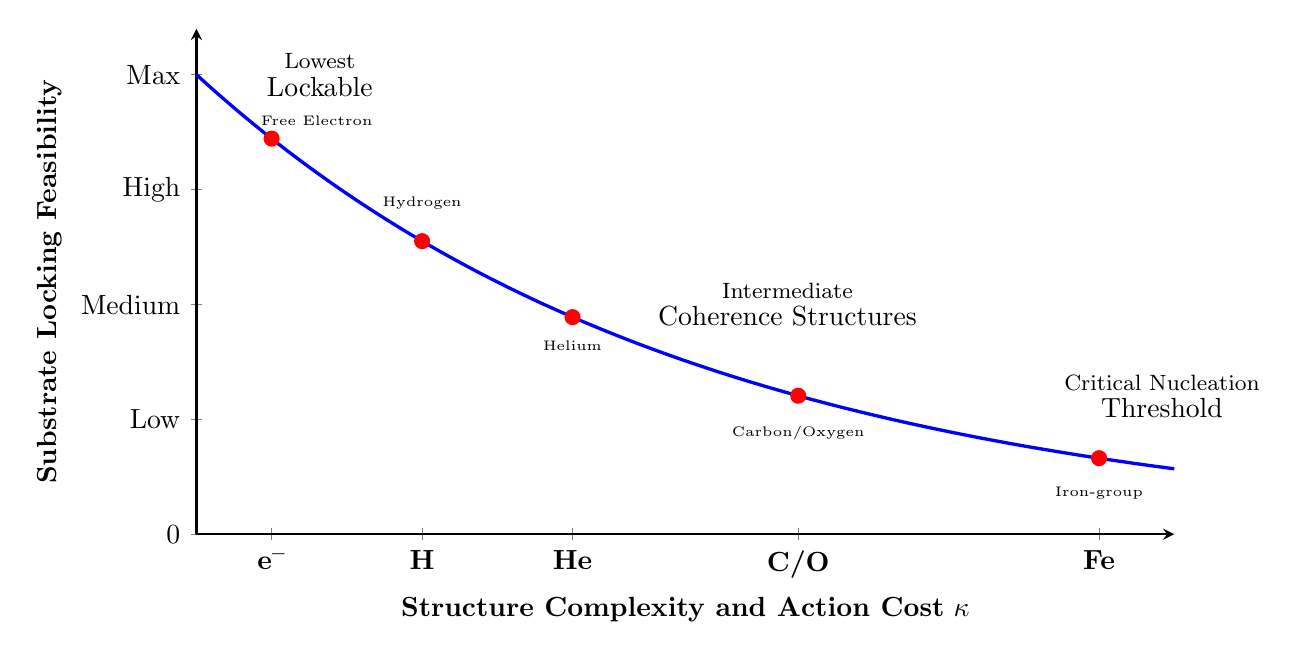
\begin{tikzpicture}

  % Axes
  \begin{axis}[
    width=14cm,
    height=8cm,
    axis lines=left,
    xlabel={\textbf{Structure Complexity and Action Cost} $\kappa$},
    ylabel={\textbf{Substrate Locking Feasibility}},
    ymin=0, ymax=1.1,
    xmin=0, xmax=6.5,
    xtick={0.5, 1.5, 2.5, 4.0, 6.0},
    xticklabels={\textbf{e\textsuperscript{--}}, \textbf{H}, \textbf{He}, \textbf{C/O}, \textbf{Fe}},
    ytick={0,0.25,0.5,0.75,1.0},
    yticklabels={0, Low, Medium, High, Max},
    enlargelimits=false,
    clip=false,
    domain=0:6.5,
    samples=100,
    smooth,
    thick
  ]

  % Feasibility curve: starts high, falls with increasing complexity
  \addplot[blue, very thick] {exp(-0.3*x)};

  % Markers for elements
  \addplot[only marks, mark=*, mark size=2.5pt, color=red] coordinates {
    (0.5, {exp(-0.3*0.5)})
    (1.5, {exp(-0.3*1.5)})
    (2.5, {exp(-0.3*2.5)})
    (4.0, {exp(-0.3*4.0)})
    (6.0, {exp(-0.3*6.0)})
  };

  % Labels for regions
  \node[align=center, anchor=west] at (axis cs:0.4,1.0) {\footnotesize Lowest\\[-2pt]Lockable};
  \node[align=center, anchor=west] at (axis cs:3.0,0.50) {\footnotesize Intermediate\\[-2pt]Coherence Structures};
  \node[align=center, anchor=west] at (axis cs:5.7,0.3) {\footnotesize Critical Nucleation\\[-2pt]Threshold};

  % Annotations for elements
  \node at (axis cs:0.8,0.90) {\tiny Free Electron};
  \node at (axis cs:1.5,0.72) {\tiny Hydrogen};
  \node at (axis cs:2.5,0.41) {\tiny Helium};
  \node at (axis cs:4.0,0.22) {\tiny Carbon/Oxygen};
  \node at (axis cs:6.0,0.09) {\tiny Iron-group};

  \end{axis}

\end{tikzpicture}
\caption{Minimal Locking Configurations Spectrum. Locking feasibility declines with increasing structural complexity and action burden. Lighter elements (left) lie deep in the nucleation wedge; heavier elements approach feasibility boundaries.}
\label{fig:locking}
\end{figure}


\subsubsection*{Inertial Drag as Structural Persistence}

In QSD, motion is implemented by re-locking a structure across successive ticks. CPA fields from recent collapse events inhibit immediate re-locking in the same direction, creating a form of structural drag. This \emph{inertial delay} emerges because the substrate region has not yet recovered sufficient coherence availability. The result is a causal form of resistance—not due to an external force, but from local feasibility limits imposed by structural history.

\subsubsection*{CPA Saturation and Recovery Lag}

Regions subjected to repeated collapse accumulate CPA residues that slow coherence recovery. As these distortions accumulate, the substrate can become \emph{saturated}, suppressing further re-locking. In such zones, collapse may divert into bleed, rupture, or degraded offload modes. This saturation dynamic mimics decoherence or entropy growth but arises entirely from deterministic substrate behavior. See Figure \ref{fig:cpa}.


\begin{figure}[ht]
\centering
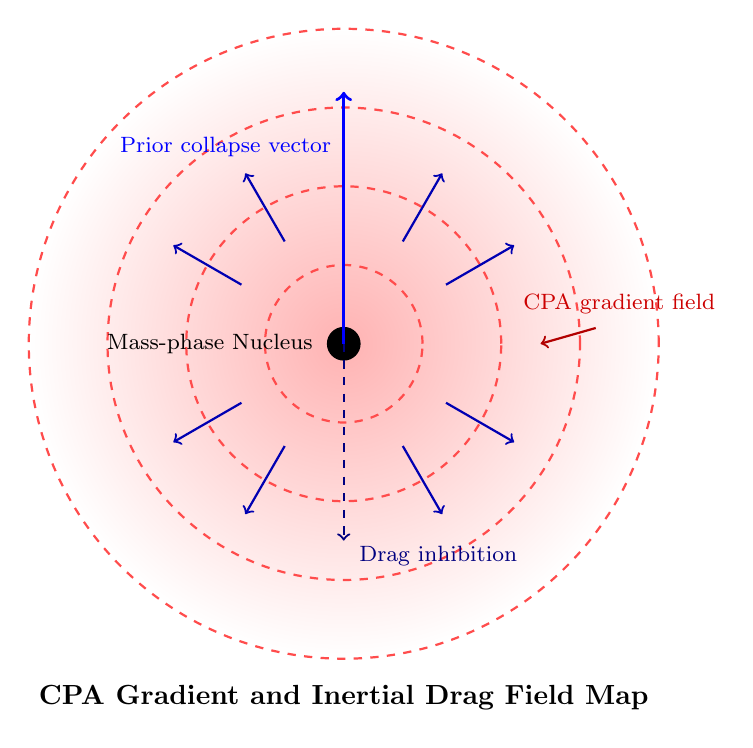
\begin{tikzpicture}[scale=1.0, thick]

  % Define the color gradient for CPA intensity
  \shade[inner color=red!30, outer color=white]
    (0,0) circle (4);

  % Draw concentric CPA gradient rings
  \foreach \r in {1,2,3,4} {
    \draw[red!70, dashed] (0,0) circle (\r);
  }

  % Mass-phase core
  \filldraw[black] (0,0) circle (0.2);
  \node at (-1.7,0.0) {\footnotesize Mass-phase Nucleus};

  % Phase drag vectors (CPA memory tail)
  \foreach \angle in {30, 60, 120, 150, 210, 240, 300, 330} {
    \draw[->, thick, blue!70!black] 
      ({cos(\angle)*1.5}, {sin(\angle)*1.5}) 
      -- ({cos(\angle)*2.5}, {sin(\angle)*2.5});
  }

  % Inertial drag suppression (opposite of motion)
  \draw[->, very thick, blue] (0,0) -- (0,3.2);
  \node[blue] at (-1.5,2.5) {\footnotesize Prior collapse vector};

  \draw[->, thick, blue!50!black, dashed] (0,0) -- (0,-2.5);
  \node[blue!50!black] at (1.2,-2.7) {\footnotesize Drag inhibition};

  % CPA bias labels
  \node[red!80!black] at (3.5, 0.5) {\footnotesize CPA gradient field};
  \draw[->, red!70!black] (3.2, 0.2) -- (2.5,0);

  % Region label
  \node at (0,-4.5) {\textbf{CPA Gradient and Inertial Drag Field Map}};

\end{tikzpicture}
\caption{CPA gradients (red) radiate from the collapse source, while blue vectors illustrate phase drag and re-lock inhibition. Prior collapse direction creates persistent asymmetry in re-lock feasibility.}
\label{fig:cpa}
\end{figure}



\subsubsection*{Observable Structural Signatures}

CPA field dynamics offer testable predictions across experimental and astrophysical regimes:

\begin{itemize}
    \item \textbf{Directional Emission Skew:} Collapse products exhibit angular bias due to inherited phase asymmetries.
    \item \textbf{Inertial Drag:} Resistance to acceleration or redirection arises from delayed re-locking along previously collapsed directions.
    \item \textbf{Asymmetric Debris Profiles:} High-energy ejecta patterns reflect collapse history, not just local thermodynamics.
    \item \textbf{Signal Damping and Coherence Fade:} CPA saturation reduces re-lock contrast and delays subsequent structural formation.\footnote{See Appendix~\ref{app:sn1987a} for SN~1987A halo diffusion and coherence decay as possible CPA-linked effects.}
\end{itemize}

\subsubsection*{Memory as a Constraint, Not a Process}

In QSD, memory is embodied in structure—not computation. CPA fields shape collapse feasibility by preserving geometric influence from past intervals. The substrate does not “reset” between ticks; each CI is conditioned by the remnants of prior configurations. This structural continuity enforces directional persistence, collapse asymmetry, and inertial lag as natural outcomes of finite coherence capacity and causal pacing.


%%%%%%%%%%%%%%%%%%%%%%%%%%%%%%%%%%%%%%%%%%
\section{Conclusion}

This work has advanced a first-principles model of mass-phase nucleation within the framework of Quantum Substrate Dynamics (QSD), establishing a structural and causal foundation for mass, quantization, and gravitational behavior. By formalizing the roles of Causality Intervals (CI), Collapse Boundaries (CB), and Quantum Emission Opportunities (QEO), we reframed mass not as an intrinsic attribute or a field-generated value, but as a persistent coherence structure—one that survives repeated substrate feasibility tests across discrete resolution cycles.

Central to this framework is the idea that energy must be structurally resolved at each CI through re-locking, emission, rupture, or capture. This enforces a bounded feasibility region—defined by substrate yield limits, coherence-action capacity, scalar recovery time, and structural overlap—that constrains which configurations may persist. Only those falling within this “Goldilocks window” can re-lock and accumulate as mass-phase structures.

A key result of this model is the reinterpretation of Planck’s constant \( h \) as the maximum coherent offload per interval—a direct expression of the substrate’s structural capacity. Likewise, the gravitational constant \( G \) is retained in its predictive form but redefined as a compliance coefficient that governs nucleation feasibility rather than spacetime curvature. In this way, QSD recovers all classical and relativistic predictions while supplying a deeper substrate-based origin for their emergence.

The introduction of a substrate action principle further grounds QSD in variational dynamics, allowing coherent evolution to be derived from extremal action under feasibility constraints. This frames quantization not as a postulate but as a structural necessity imposed by substrate limits.

The theory yields testable predictions across multiple domains. Coherence-shell banding, spectral emission combs, nucleation thresholds, and CPA-driven asymmetries provide falsifiable observables in astrophysical, quantum, and condensed-matter contexts. These signatures arise not from hidden variables or modified equations, but from structural resolution laws already implicit in the substrate framework.

In summary, this work repositions mass as a consequence of structural retention under causal constraints. What persists through repeated collapse is what qualifies as matter. Quantization arises from substrate capacity, not axioms; gravitational behavior from coherence gradients, not geometry. The coherence envelope becomes the fundamental unit of persistence—and mass its retained expression. Together, these insights open a pathway toward a unified substrate theory where quantum structure, relativistic behavior, and gravitational interaction all emerge from the same coherence-governed foundation.




%%%%%%%%%%%%%%%%%%%%%%%%%%%%%%%%%%%%%%%%%%
\vspace{6pt} 

%%%%%%%%%%%%%%%%%%%%%%%%%%%%%%%%%%%%%%%%%%
%% optional
%\supplementary{The following supporting information can be downloaded at:  \linksupplementary{s1}, Figure S1: title; Table S1: title; Video S1: title.}

% Only for journal Methods and Protocols:
% If you wish to submit a video article, please do so with any other supplementary material.
% \supplementary{The following supporting information can be downloaded at: \linksupplementary{s1}, Figure S1: title; Table S1: title; Video S1: title. A supporting video article is available at doi: link.}

% Only used for preprtints:
% \supplementary{The following supporting information can be downloaded at the website of this paper posted on \href{https://www.preprints.org/}{Preprints.org}.}

% Only for journal Hardware:
% If you wish to submit a video article, please do so with any other supplementary material.
% \supplementary{The following supporting information can be downloaded at: \linksupplementary{s1}, Figure S1: title; Table S1: title; Video S1: title.\vspace{6pt}\\
%\begin{tabularx}{\textwidth}{lll}
%\toprule
%\textbf{Name} & \textbf{Type} & \textbf{Description} \\
%\midrule
%S1 & Python script (.py) & Script of python source code used in XX \\
%S2 & Text (.txt) & Script of modelling code used to make Figure X \\
%S3 & Text (.txt) & Raw data from experiment X \\
%S4 & Video (.mp4) & Video demonstrating the hardware in use \\
%... & ... & ... \\
%\bottomrule
%\end{tabularx}
%}

\section*{Statements and Declarations}
\subsection*{Funding}  
The author received no financial support for the research, authorship, or publication of this article.
The author has no relevant financial or non-financial interests to disclose.

\subsection*{Competing Interests}  
The author declares no competing interests.

\subsection*{Author Contributions}  
The author solely conceived, developed, and wrote the manuscript, including all theoretical content, references, and formatting.

\subsection*{Data Availability}  
No datasets were generated or analyzed during the current study. All references are publicly available.

\subsection*{Ethical Approval}  
Not applicable.


%%%%%%%%%%%%%%%%%%%%%%%%%%%%%%%%%%%%%%%%%%
%% Optional

%% Only for journal Encyclopedia
%\entrylink{The Link to this entry published on the encyclopedia platform.}

\abbreviations{Abbreviations}{
The following abbreviations are used in this manuscript:
\\

\noindent
\begin{tabular}{@{}ll}
QSD   & Quantum Substrate Dynamics \\
CI    & Causality Interval (minimum recoverable coherence cycle) \\
CB    & Collapse Boundary (end-state of a CI, structural re-lock) \\
QEO   & Quantum Emission Opportunity (conditional offload at CB) \\
CIC   & Coherence–Information Capacity (bound on recoverable structure) \\
\( c_s \) & Scalar coherence recovery speed (temporal mode) \\
\( c_t \) & Transverse coherence propagation speed (spatial mode) \\
\( L_{\text{coh}} \) & Effective coherence support length \\
\( L_n \) & Quantized coherence envelope length (nth mode) \\
\( E_\star \) & Structural energy threshold for nucleation stability \\
\( \kappa \) & Substrate compliance constant (curvature–tension ratio) \\
\( \tau \) & Scalar recovery interval associated with CI pacing \\
\( \Delta\nu \) & Spectral comb spacing \( = c_s / L_{\text{coh}} \) \\
\( k_{\text{coh}} \) & Coherence wavenumber \( \sim 2\pi/L_{\text{coh}} \) \\
\( R(t) \) & Recovery function for post-collapse coherence restoration \\
\( P_{\text{offload}}(t) \) & Power released during quantized emission offload \\
\( \rho(\vec{r},t) \) & Local coherence tension density \\
\end{tabular}

}



%%%%%%%%%%%%%%%%%%%%%%%%%%%%%%%%%%%%%%%%%%
%% Optional
\appendixtitles{no} % Leave argument "no" if all appendix headings stay EMPTY (then no dot is printed after "Appendix A"). If the appendix sections contain a heading then change the argument to "yes".
\appendixstart
\appendix
\section[\appendixname~\thesection]{Glossary of Core Substrate Dynamics}
\label{app:glossary}
\subsection[\appendixname~\thesubsection]{}

To aid first-time readers and clarify foundational assumptions, this glossary summarizes the minimal causal architecture of Quantum Substrate Dynamics (QSD). These core terms describe the substrate-driven process through which emission, collapse, and persistent mass-phase structure emerge.

\begin{description}

  \item[CI — Causality Interval.]
  The fundamental temporal unit of substrate evolution.  
  A Causality Interval spans a finite duration  
  \[
  \tau = \frac{L_{\mathrm{coh}}}{c_s},
  \]
  during which local coherence may evolve freely. At the end of each CI, structural resolution is enforced. Waveforms must either offload, collapse, or lock into a persistent configuration.

  \item[CB — Collapse Boundary.]  
  The mandatory resolution event at the end of a CI.  
  At the CB, all unresolved phase structure must be resolved via one of four outcomes:  
  radiative emission, structural transfer, rupture, or stable mass-phase capture.  
  The CB is a substrate-imposed enforcement of causal closure, not an optional transition.

  \item[QEO — Quantum Emission Opportunity.]  
  The conditionally available event at each CB, where unresolved phase structure may be serialized into discrete emissions.  
  If the configuration is not geometrically compatible with persistence, the QEO produces radiation or rupture.  
  If all feasibility constraints are satisfied, the QEO can yield a locked mass-phase. Thus, nucleation is a subset of QEO resolution.

  \item[CIC — Coherence–Information Capacity.]  
  The maximum coherent action that can be supported across one CI:  
  \[
  A_{\max} = E_{\mathrm{P}} \cdot \tau = \frac{c_t^4}{G}\cdot\frac{L_{\mathrm{coh}}}{c_s}.
  \]  
  This sets an upper bound on structural complexity.  
  If the maintenance action \( A_\kappa(L) \) required to sustain a structure exceeds this threshold, coherence fails and the structure cannot persist.

  \item[CPA — Causal Phase Aftereffect.]  
  The residual memory field left behind by collapse or emission.  
  CPA fields encode the directional phase bias and depleted coherence footprint of prior configurations.  
  They influence subsequent evolution by biasing the phase landscape for future CIs, and may give rise to emission skew, directional drag, or nucleation banding.

  \item[Tick Map.]  
  A symbolic trace of the discrete pathway a coherence region follows across successive CIs.  
  Typical transitions include:
  \[
  \text{seed} \rightarrow \text{grow} \rightarrow \{\text{emit},\,\text{bleed},\,\text{rupture},\,\text{lock}\},
  \]
  where each outcome is selected by the local feasibility conditions.  
  Tick maps visualize the resolution logic of structural evolution in QSD.

  \item[Goldilocks Window.]  
  The bounded feasibility region where persistence as a mass-phase structure becomes possible.  
  Below this window, coherence-action is insufficient to retain the structure, leading to bleed.  
  Above it, the energy exceeds substrate yield or rate limits, causing rupture.  
  Only within this window can mass-phase nucleation succeed and remain stable.

\end{description}

\subsection[\appendixname~\thesubsection]{}
The CI–CB–QEO–CIC–CPA cycle defines the minimal structural grammar of Quantum Substrate Dynamics.  
Each CI enforces causality through a Collapse Boundary; QEOs offer resolution pathways; CIC bounds set coherence retention limits; and CPA fields carry structural memory.  
The Goldilocks window delineates which configurations can persist across time.  
Together, these terms establish the substrate law from which mass, emission, and inertial structure naturally arise.

%%%%%%%%%%%%%%%%%%%%%%%%%%%%%%%%%%%%%%%%%%%%%%%
%%%%%%%%%%%%%%%%%%%%%%%%%%%%%%%%%%%%%%%%%%%%%%%
\section[\appendixname~\thesection]{Toy Model: Nucleation Feasibility Wedge and Critical Length \texorpdfstring{$L_n$}{Ln}}
\label{app:toy}
%%%%%%%%%%%%%%%%%%%%%%%%%%%%%%%%%%%%%%%%%%%%%%

\subsection[\appendixname~\thesubsection]{Overview}
This appendix presents a conceptual 1D toy model that illustrates how nucleation feasibility emerges from constraint intersections in Quantum Substrate Dynamics (QSD). Using a simplified energy scaling law, we derive a closed-form expression for the critical length \( L_n \) and define the nucleation wedge in the \((E, L)\) space. The aim is not to describe real substrate dynamics, but to provide an intuitive visualization of the constraint-based geometry central to QSD.

\subsection{Model Setup}
Assume a single admissible envelope mode with coherence scale \( L \equiv L_{\mathrm{coh}} \). Let the per–CI binding energy scale with coherence size as:
\begin{equation}
E_\star(L) = E_0 \left(\frac{L}{L_{\mathrm{ref}}}\right)^{-q}, \qquad q > 0,
\label{eq:toy-Estar}
\end{equation}
where \( E_0 \) and \( L_{\mathrm{ref}} \) set the energy and length scales.

Nucleation feasibility requires satisfaction of both rate and yield constraints:
\begin{equation}
\frac{\eta^{-1} E_\star(L)}{\tau} \le c^5, \qquad \eta^{-1} E_\star(L) < E_{\mathrm{P}}(L),
\quad \text{with} \quad \tau = \frac{L}{c_s}, \quad E_{\mathrm{P}}(L) = \frac{c_t^4}{G} L.
\label{eq:toy-bounds}
\end{equation}
These simplify to:
\begin{equation}
\eta^{-1} E_\star(L) \le m_\ast L,
\qquad m_\ast = \min\left\{ \frac{c^5}{c_s}, \frac{c_t^4}{G} \right\},
\label{eq:mstar}
\end{equation}
so \( E_\star(L) \) must lie beneath the tighter of two linear ceilings.

\subsection[\appendixname~\thesubsection]{Wedge Geometry and Critical Length}
In \((\log L, \log E)\) space, \eqref{eq:toy-Estar} is a line of slope \(-q\), and the ceiling \( \eta m_\ast L \) is slope \(+1\). Their intersection yields:
\begin{equation}
L_n = L_{\mathrm{ref}} \left( \frac{\eta E_0}{m_\ast L_{\mathrm{ref}}^{q+1}} \right)^{1/(q+1)}.
\label{eq:Ln}
\end{equation}
Below \( L_n \), nucleation fails; above it, feasibility is achieved.

\paragraph*{Remark (Active Ceiling)}
If \( c^5/c_s < c_t^4/G \), then rate dominates: \( m_\ast = c^5/c_s \). Otherwise, yield governs: \( m_\ast = c_t^4/G \).

\subsection[\appendixname~\thesubsection]{Persistence and CIC Constraint}
To ensure persistence, per-CI coherence maintenance must satisfy the CIC bound:
\begin{equation}
A_\kappa(L) = A_0 \left(\frac{L}{L_{\mathrm{ref}}}\right)^{-r}, \qquad r > 0,
\end{equation}
\begin{equation}
L \ge L_{\min}^{\mathrm{CIC}} = L_{\mathrm{ref}} \left( \frac{A_0}{\eta h} \right)^{1/r}.
\label{eq:LminCIC}
\end{equation}
With curvature limit \( L \le L_{\max}^{\mathrm{geom}} \), persistence requires:
\begin{equation}
L \in \left[ L_{\min}^{\mathrm{CIC}}, L_{\max}^{\mathrm{geom}} \right], \quad \text{and} \quad E_\star(L) \le \eta m_\ast L.
\end{equation}

\subsection[\appendixname~\thesubsection]{Numerical Example (Dimensionless)}
Let \( m_\ast = 1 \), \( L_{\mathrm{ref}} = 1 \), \( q = 1 \), \( \eta = 0.3 \), \( E_0 = 0.3 \). Then:
\[
L_n = \left( 0.3 \times 0.3 \right)^{1/2} = 0.30.
\]
For CIC: \( r = 2 \), \( A_0 / (\eta h) = 0.25 \), so:
\[
L_{\min}^{\mathrm{CIC}} = (0.25)^{1/2} = 0.50.
\]
Here, \( L_n < L_{\min}^{\mathrm{CIC}} \): nucleation is feasible but unstable. Tuning \( \eta \) or \( A_0 \) shifts the crossover.

\subsection[\appendixname~\thesubsection]{Schematic Wedge}
Define:
\[
\mathcal{W} = \left\{ (L, E): E \le \eta m_\ast L \right\},
\]
with \( E_\star(L) = E_0(L/L_{\mathrm{ref}})^{-q} \). Their intersection at \( L_n \) shows the wedge's onset. Plotting on log–log axes reveals the geometric picture of constraint-driven nucleation.

\paragraph*{Summary}
This toy model clarifies the emergence of a bounded feasibility window defined by rate, yield, and CIC constraints. Though simplified, it reinforces QSD’s structural claim: that persistence arises not from postulates but from causal compatibility across coherence scales.


%%%%%%%%%%%%%%%%%%%%%%%%%%%%%%%%%%%%%%%%%%
\section[\appendixname~\thesection]{Derivation Details: Inequality Bounds and Compactness of \texorpdfstring{$W_n$}{Wn}}
%%%%%%%%%%%%%%%%%%%%%%%%%%%%%%%%%%%%%%%%%%%%%%%
%%%%%%%%%%%%%%%%%%%%%%%%%%%%%%%%%%%%%%%%%%
\subsection[\appendixname~\thesubsection]{Overview}

This appendix collects the derivation details for the nucleation feasibility set \( W_n \), which defines where coherence-locked mass structures are allowed. It provides a compact, bounded region in coherence-length space, ensuring the existence of critical nucleation thresholds \( L_n \) under well-defined structural constraints.

\subsection[\appendixname~\thesubsection]{Three governing bounds}
A coherence envelope of size \( L \equiv L_{\mathrm{coh}} \) must simultaneously satisfy three constraints:

\begin{enumerate}
  \item \textbf{Rate Bound (Offload Constraint):}
  \begin{equation}
  \frac{E_\star(L)}{\tau} \;\le\; \eta\,c^5, \qquad \text{where } \tau = \frac{L}{c_s}.
  \end{equation}
  This ensures that the per-interval energy accumulation does not exceed the substrate’s causal offload capacity.

  \item \textbf{Storage Bound (Yield Constraint):}
  \begin{equation}
  E_\star(L) \;\le\; \eta\,E_{\mathrm{P}}(L), \qquad E_{\mathrm{P}}(L) = \frac{c_t^4}{G} L.
  \end{equation}
  This ensures the stored energy remains within the local yield limit imposed by the substrate at scale \( L \).

  \item \textbf{CIC Bound (Structural Stability Constraint):}
  \begin{equation}
  A_\kappa(L) \;\le\; \eta\,h.
  \end{equation}
  Here \( A_\kappa(L) \) is the per-cycle structural action. This constraint defines the lower size limit: below it, coherence cannot be structurally maintained.
\end{enumerate}

Together, these define the feasible wedge:
\begin{equation}
W_n \;=\; \left\{ L > 0 \;\bigg|\; 
E_\star(L) \le \min\!\left(\eta\,\frac{c^5}{c_s}L,\; \eta\,\frac{c_t^4}{G}L\right), \quad
A_\kappa(L) \le \eta h \right\}.
\end{equation}

\subsection[\appendixname~\thesubsection]{Continuity of the bounding curves}
Both the envelope requirement \( E_\star(L) \) and maintenance action \( A_\kappa(L) \) are assumed continuous in \( L \), reflecting smooth physical demands. The ceiling functions \( \eta c^5 L / c_s \) and \( \eta c_t^4 L / G \) are linear and continuous. Therefore, the full set of constraints is composed of continuous inequality relations over \( L > 0 \).

\subsection[\appendixname~\thesubsection]{Compactness of the feasible wedge}
To ensure existence of a well-defined nucleation region, we demonstrate that \( W_n \) is compact:

\begin{itemize}
  \item \textbf{Lower bound:}  
  The CIC constraint imposes a minimum coherence length:
  \[
  L \;\ge\; L_{\min}^{\mathrm{CIC}}.
  \]

  \item \textbf{Upper bound:}  
  Geometric or rupture limits (from curvature or coherence loss) impose a maximum length:
  \[
  L \;\le\; L_{\max}^{\mathrm{geom}}.
  \]

  \item \textbf{Closed region:}  
  Since the inequalities are defined by continuous functions, their sublevel sets are closed. Therefore, the region between the lower and upper bounds is closed and bounded.
\end{itemize}

Thus, the feasible domain satisfies:
\begin{equation}
W_n \;\subseteq\; \left[ L_{\min}^{\mathrm{CIC}},\; L_{\max}^{\mathrm{geom}} \right],
\end{equation}
and is compact by the Heine–Borel theorem.

\subsection[\appendixname~\thesubsection]{Existence of a critical nucleation length}
If \( E_\star(L) \) decreases with \( L \) (as expected for complex structures) and the ceilings increase linearly with \( L \), the two curves will intersect at least once in the compact wedge \( W_n \). This intersection defines a critical coherence length:
\[
L_n \quad\text{such that}\quad E_\star(L_n) = \min\!\left(\eta\,\frac{c^5}{c_s}L_n,\; \eta\,\frac{c_t^4}{G}L_n\right).
\]
Compactness ensures that such an \( L_n \) exists and lies within the physically admissible window, forming the threshold for nucleation feasibility.

\subsection[\appendixname~\thesubsection]{Summary}
The feasibility region \( W_n \) is compact, continuous, and well-posed under the QSD framework. This guarantees that nucleation conditions produce physically consistent critical lengths, offering a robust foundation for structural analysis and observational validation.

%%%%%%%%%%%%%%%%%%%%%%%%%%%%%%%%%%%%%%%%%%
\section[\appendixname~\thesection]{Observational Signatures: Coherence Shells in SN 1987A}
\label{app:sn1987a}
\subsection[\appendixname~\thesubsection]{Overview}

Supernova 1987A provides a rare observational testbed for coherence-locked mass nucleation due to its proximity, well-documented evolution, and high-resolution imaging across multiple spectral bands. Within the framework of Quantum Substrate Dynamics (QSD), the expanding ejecta and ring structures are interpreted not as turbulent hydrodynamic remnants, but as phase-locked coherence shells formed at discrete Collapse Boundaries (CBs).

The prominent \emph{inner ring}, located approximately 0.66 light-years from the explosion site, displays sharply resolved emission profiles in oxygen, nitrogen, hydrogen, and sulfur. While traditionally attributed to pre-supernova mass loss, QSD offers an alternative interpretation: the ring and nested shells are coherence-defined layers, each nucleated when local substrate conditions met the structural feasibility constraints at a Causality Interval (CI) tick.

\subsection[\appendixname~\thesubsection]{Coherence-Locked Shell Formation}

Under QSD, heavy elements such as iron-group nuclei nucleate near the core, where the scalar compression exceeds both yield and coherence-action thresholds. As the collapse wave propagates outward and the scalar field weakens, lighter elements nucleate in concentric bands—each satisfying the CB feasibility constraints at a successively lower coherence capacity. Marginal regions that fall outside the Goldilocks window produce emission-only zones or metastable coherence bleed.

This coherence-layering model leads to the following observational predictions:

\begin{itemize}
  \item \textbf{Radial Spectral Banding:} Discrete shell spacing should produce peaks in radial Fourier transforms of emission intensity, with spatial frequency \( k_{\mathrm{coh}} \sim 2\pi / L_{\mathrm{coh}} \), where \( L_{\mathrm{coh}} \) is the coherence scale at which the shell nucleated.
  
  \item \textbf{Cross-Band Scale Locking:} The same radial frequencies should appear across diverse observational bands—optical line profiles, mid-infrared dust emissions, and ALMA molecular tracers—reflecting common CB pacing at the substrate level.

  \item \textbf{Substructure and Stratification:} Fine-grained sub-banding within elemental layers is expected due to repeated CI re-lock cycles, manifesting as nested shells or polarization-aligned substructures.

  \item \textbf{Rupture-Edge Gradients:} Beyond each coherent shell, emission zones should become diffuse and element-poor, marking the outer failure edge where substrate coherence could not lock. This should appear as a sharp abundance cutoff followed by extended emission halos.
\end{itemize}

\subsection[\appendixname~\thesubsection]{Alignment with SN 1987A Observations}

These predictions are increasingly supported by observations of SN 1987A’s ejecta structure:

\begin{itemize}
  \item High-resolution imaging (e.g., HST/STIS) reveals chemically stratified shells with discrete radii and non-turbulent morphology \cite{fransson2015,larsson2016}.
  \item ALMA maps of CO and SiO show clumped molecular emission consistent with coherence-based ring formation \cite{alma2017,abellan2020}.
  \item X-ray hotspot progression and infrared light echoes trace sequential ring activations, suggestive of re-lock memory sequences rather than stochastic instabilities.
\end{itemize}

These observations align with QSD’s interpretation of mass nucleation as a **quantized structural phenomenon** governed by substrate constraints. The existence of discrete, composition-dependent shells, reproducible radial spacing, and directional symmetry point to causal phase-locking rather than explosive randomness.

\subsection[\appendixname~\thesubsection]{Implications and Testing}

SN 1987A thus serves as a candidate falsification site for QSD’s coherence-nucleation model. Further observational tests include:

\begin{itemize}
  \item Radial FFT analyses across emission bands to detect quantized shell spacing.
  \item Cross-modal spectral alignment (optical/IR/ALMA) at coherence frequencies.
  \item Comparison of elemental abundance falloff with rupture-gradient predictions.
\end{itemize}

These tests could distinguish QSD’s deterministic coherence-shell model from standard hydrodynamic or turbulence-driven models. If the predicted radial harmonics and decay zones are confirmed, SN 1987A may offer the first empirical validation of collapse-driven structural retention in a conserved substrate framework.

%%%%%%%%%%%%%%%%%%%%%%%%%%%%%%%%%%%%%%%%%%%
%%%%%%%%%%%%%%%%%%%%%%%%%%%%%%%%%%%%%%%%%%
\section[\appendixname~\thesection]{Experimental Implications and Falsifiable Predictions}
\label{app:experimental}
\subsection[\appendixname~\thesubsection]{Overview}

Quantum Substrate Dynamics (QSD) makes structurally anchored, falsifiable predictions based on collapse pacing, substrate feasibility limits, and coherence-locked resolution. These signatures are not parameter-tuned artifacts but direct consequences of the theory’s causal framework.

\paragraph{Collapse Pacing and Spectral Quantization.}
Each substrate region evolves over discrete Causality Intervals (CI) of duration
\[
\tau = \frac{L_{\mathrm{coh}}}{c_s},
\]
with each Collapse Boundary (CB) enforcing structural resolution. This introduces a quantized offload rhythm, predicting spectral combs with spacing
\[
\Delta \nu = \frac{c_s}{L_{\mathrm{coh}}}.
\]
These combs should appear in FFTs of pulsar, plasma, or supernova spectra, reflecting serialized structural offload—not mode interference or thermal broadening.

\paragraph{Radial Banding and Layered Morphology.}
Mass nucleation produces concentric shells at coherence-defined radii. Observable consequences include:
\begin{itemize}
  \item Discrete elemental zonation (e.g., in SN 1987A),
  \item Radial banding in emission and density profiles,
  \item Nested shell structures across optical, IR, and molecular bands.
\end{itemize}
These alignments are not thermodynamic in origin, but reflect substrate pacing and collapse thresholds.

\paragraph{Directional Memory (CPA Residue).}
Collapse leaves behind Causal Phase Aftereffects (CPA)—substrate-encoded structural memory that biases subsequent evolution. Testable effects include:
\begin{itemize}
  \item Emission anisotropy or skew near collapse sites,
  \item Suppression or delay of nucleation in CPA-saturated regions,
  \item Directional dependence in re-lock probability.
\end{itemize}
Such effects can be probed via time-resolved cavity experiments or pulsed plasma systems.

\paragraph{Early-Stage Feasibility in Confined Systems.}
The onset of nucleation can be indirectly tested in bounded, coherence-sensitive regimes:
\begin{itemize}
  \item Plasma confinement under dynamic compression (yield crossing),
  \item High-Q optical cavities (coherence reflection thresholds),
  \item Triggered quantum dot systems (collapse gating windows).
\end{itemize}
Controlled tuning of coherence scale or pacing (\(L_{\mathrm{coh}}, \tau\)) allows experimental access to QSD constraint regimes.

\paragraph{Substrate Yield Limits}
The QSD yield threshold,
\[
E_{\mathrm{P}}(L) = \frac{c_t^4}{G} L,
\]
acts as a local energy ceiling. When exceeded, collapse transitions to rupture. Observable effects may include:
\begin{itemize}
  \item Fixed-size emission zones,
  \item Sudden envelope blowouts,
  \item Breakdown of coherent oscillation under overload.
\end{itemize}
This provides a testable path to infer \( G \) and \( c_t \) from empirical rupture behavior.

\paragraph{Outlook.}
All predictions arise from the structural grammar of QSD: enforced re-locks, coherence pacing, and substrate-bound feasibility. No statistical assumptions or probabilistic collapse are invoked. If coherence structures fail to meet these constraints, they must rupture, decay, or vanish—providing a crisp falsifiability condition and a testbed for probing the foundational behavior of physical structure.


%%%%%%%%%%%%%%%%%%%%%%%%%%%%%%%%%%%%%%%%%%
\section[\appendixname~\thesection]{Unified Implications: Gravity, Mass Spectrum, and Cosmological Structure}
\label{app:unified}
\subsection[\appendixname~\thesubsection]{Overview}

The structural model of mass-phase nucleation in Quantum Substrate Dynamics (QSD) yields unified consequences across physical regimes. Without invoking fields, curvature, or particle types, QSD explains gravity, the mass spectrum, and large-scale structure as outcomes of substrate-constrained coherence resolution.

\paragraph{Gravity as Substrate Saturation Gradient.}
Gravitational behavior arises from local substrate depletion. Each nucleation event irreversibly captures coherence, reducing scalar recovery headroom and modifying effective compliance:
\[
G_{\mathrm{eff}}(\mathbf{x},t) = G \cdot R^{-1}(\mathbf{x},t).
\]
This creates a persistent substrate tension gradient—a coherence slope—that biases nearby re-locking and motion. Gravity is thus reframed as a structural response to phase depletion, not as metric curvature.

\paragraph{Discrete Mass Spectrum from Feasibility Constraints.}
Only certain coherence configurations satisfy all feasibility bounds:
\[
A_\kappa(L) \le \eta\,A_{\max}(L), \quad \Delta E < E_{\mathrm{P}}(L), \quad \Gamma \in [0,1].
\]
These constraints select a discrete set of survivable mass-phase structures—each with quantized energy, stability, and emission profile. The nuclear mass spectrum emerges from this bounded feasibility window, not from anthropic tuning or spontaneous symmetry breaking.

\paragraph{Spectral Lines as Collapse-Encoded Emissions.}
Each stable structure has a coherence scale \( L_{\mathrm{coh}} \), setting its emission frequency:
\[
\Delta \nu = \frac{c_s}{L_{\mathrm{coh}}}.
\]
Spectral lines are serialized collapse outputs from the internal phase geometry—not probabilistic transitions between energy levels. This coherence-based quantization explains both atomic and nuclear spectra in terms of substrate timing and structure.

\paragraph{Cosmic Structure as Frozen Collapse Memory.}
Successive CBs across cosmological time create nested coherence gradients and shell structures. These gradients persist and modulate large-scale matter organization. Features such as:
\begin{itemize}
  \item Galaxy rotation asymmetries,
  \item Filament alignment and void spacing,
  \item Power spectrum features in CMB,
\end{itemize}
may arise from non-geometric coherence drag—not from cold dark matter halos or modified gravity models.

\paragraph{Summary}
QSD unifies gravity, mass, spectrum, and cosmic structure as expressions of the same principle: **coherence-constrained resolution** within a conserved substrate. Gravitational interaction becomes a memory gradient. Mass becomes the residual of feasibility. Spectral quantization reflects serialized offload. And cosmic morphology encodes collapse history. Each arises from local causality—not imposed laws, but emergent consequence.





%%%%%%%%%%%%%%%%%%%%%%%%%%%%%%%%%%%%%%%%%%



\isPreprints{}{% This command is only used for ``preprints''.
\begin{adjustwidth}{-\extralength}{0cm}
} % If the paper is ``preprints'', please uncomment this parenthesis.
%\printendnotes[custom] % Un-comment to print a list of endnotes

\reftitle{References}

% Please provide either the correct journal abbreviation (e.g. according to the “List of Title Word Abbreviations” http://www.issn.org/services/online-services/access-to-the-ltwa/) or the full name of the journal.
% Citations and References in Supplementary files are permitted provided that they also appear in the reference list here. 

%=====================================
% References, variant A: external bibliography
%=====================================
% \bibliography{your_external_BibTeX_file}

%=====================================
% References, variant B: internal bibliography
%=====================================

% ACS format
\isAPAandChicago{}{%
\begin{thebibliography}{999}
% Reference 
\bibitem{bush2025}
\textbf{Preprint.} Bush, M. (2025). Quantum Substrate Dynamics (QSD): A Relativistic Field Model of Emergent Mass, Inertia and Gravity. \textit{Preprints}, 2025060988. \url{https://doi.org/10.20944/preprints202506.0988.v1}
%Reference
\bibitem{bush-collapse-2025}
\textbf{Preprint.} Bush, M. (2025). Planck Constants as Collapse Boundaries: A Structural Framing of Quantum Evolution in Substrate Theory. \textit{Preprints}, 2025072530. \url{https://doi.org/10.20944/preprints202507.2530.v2}
% Reference
\bibitem{bush-planck-2025}
\textbf{Preprint.} Bush, M. (2025). Planck’s Constant Physically Derived Through Quantum Substrate Dynamics: A Mode-Ratio and Offload-Based Origin for Quantization and Temporal Structure. \textit{Preprints}, 2024010211. \url{https://doi.org/10.20944/preprints202401.0211.v1}
% Reference 
\bibitem{bush-coherence}
Bush, M. The Coherence Envelope: Defining the Minimum Structural Unit of Action in Quantum Substrate Dynamics. {\em Preprints} {\bf 2025}, \url{https://doi.org/10.20944/preprints202506.2353.v1}.
% Reference 
\bibitem{bush-planck-ep}
Bush, M. Planck Energy as Collapse Limit: A Structural Interpretation of $E_P$ in Quantum Substrate Dynamics. {\em Preprints} {\bf 2025}, \url{https://doi.org/10.20944/preprints202507.0080.v1}.
% Reference 
\bibitem{fransson2015}
Fransson, C., Larsson, J., Kozma, C., et al. (2015). High-Resolution Spectroscopy of SN 1987A: The Structure and Composition of the Ejecta. \textit{The Astrophysical Journal}, 806(2), L19. \url{https://doi.org/10.1088/2041-8205/806/2/L19}
% Reference 
\bibitem{larsson2016}
Larsson, J., Fransson, C., Kozma, C., et al. (2016). Three-Dimensional Mapping of the Ejecta in Supernova 1987A: Geometry and Kinematics. \textit{The Astrophysical Journal}, 833(2), 147. \url{https://doi.org/10.3847/1538-4357/833/2/147}
% Reference 
\bibitem{indebetouw2017}
Indebetouw, R., Gordon, K. D., Dwek, E., et al. (2017). ALMA Observations of the Cold Dust in the Remnant of Supernova 1987A. \textit{The Astrophysical Journal}, 848(2), 98. \url{https://doi.org/10.3847/1538-4357/aa8ccf}
% Reference 
\bibitem{abellan2020}
Abellán, F., Matsuura, M., Tziamtzis, A., et al. (2020). Three-dimensional Structure of the Ejecta in Supernova 1987A at 30 Years. \textit{Science}, 370(6513), 1450–1453. \url{https://doi.org/10.1126/science.abd0319}
% Reference 



\end{thebibliography}
}

% Chicago format (Used for journal: arts, genealogy, histories, humanities, jintelligence, laws, literature, religions, risks, socsci)
\isChicagoStyle{%
\begin{thebibliography}{999}
% Reference 1
%\bibitem[Aranceta-Bartrina(1999a)]{ref-journal}
%Aranceta-Bartrina, Javier. 1999a. Title of the cited article. \textit{Journal Title} %6: 100--10.
% Reference 2

\end{thebibliography}
}{}

% APA format (Used for journal: admsci, behavsci, businesses, econometrics, economies, education, ejihpe, games, humans, ijfs, journalmedia, jrfm, languages, psycholint, publications, tourismhosp, youth)
\isAPAStyle{%
\begin{thebibliography}{999}
% Reference 1
%\bibitem[\protect\citeauthoryear{Azikiwe \BBA\ Bello}{{2020a}}]{ref-journal}
%Azikiwe, H., \& Bello, A. (2020a). Title of the cited article. \textit{Journal Title}, \textit{Volume}(Issue), 
%Firstpage--Lastpage/Article Number.

\end{thebibliography}
}{}

% If authors have biography, please use the format below
%\section*{Short Biography of Authors}
%\bio
%{\raisebox{-0.35cm}{\includegraphics[width=3.5cm,height=5.3cm,clip,keepaspectratio]{Definitions/author1.pdf}}}
%{\textbf{Firstname Lastname} Biography of first author}
%
%\bio
%{\raisebox{-0.35cm}{\includegraphics[width=3.5cm,height=5.3cm,clip,keepaspectratio]{Definitions/author2.jpg}}}
%{\textbf{Firstname Lastname} Biography of second author}

% For the MDPI journals use author-date citation, please follow the formatting guidelines on http://www.mdpi.com/authors/references
% To cite two works by the same author: \citeauthor{ref-journal-1a} (\citeyear{ref-journal-1a}, \citeyear{ref-journal-1b}). This produces: Whittaker (1967, 1975)
% To cite two works by the same author with specific pages: \citeauthor{ref-journal-3a} (\citeyear{ref-journal-3a}, p. 328; \citeyear{ref-journal-3b}, p.475). This produces: Wong (1999, p. 328; 2000, p. 475)

%%%%%%%%%%%%%%%%%%%%%%%%%%%%%%%%%%%%%%%%%%
%% for journal Sci
%\reviewreports{\\
%Reviewer 1 comments and authors’ response\\
%Reviewer 2 comments and authors’ response\\
%Reviewer 3 comments and authors’ response
%}
%%%%%%%%%%%%%%%%%%%%%%%%%%%%%%%%%%%%%%%%%%
\isPreprints{}{\PublishersNote{}}
\isPreprints{}{% This command is only used for ``preprints''.
\end{adjustwidth}
} % If the paper is ``preprints'', please uncomment this parenthesis.
\end{document}






